\documentclass[twocolumn]{article}
% {amsart}
\usepackage[top=0.75in, left=0.65in, right=0.65in, bottom=0.6in]{geometry}

\usepackage{float}

% \usepackage{url}
% \usepackage{xurl}
\usepackage[pdftex]{hyperref}

%\usepackage{code}
\usepackage{listings}
% \usepackage{cite}
\usepackage{latexsym}
\usepackage{amsmath}
\usepackage{amssymb}
\usepackage{graphicx}
% IPA symbols. safe turns off overrides for like \! which I still want
% \usepackage[safe]{tipa}
% \usepackage{chessboard}
% \usepackage{supertabular}
\usepackage{enumitem}

% \usepackage[most]{tcolorbox}

% lets me explicitly set a. or 1. etc. as enum label
% \usepackage{enumitem}

\pagestyle{empty}

\usepackage{ulem}
% go back to italics for emphasis, though
\normalem

% do "fancy" stuff like verbatim in footnotes
\usepackage{fancyvrb}
\VerbatimFootnotes

\usepackage{natbib}
\setcitestyle{numbers,square}

\interfootnotelinepenalty=0
\setlength{\footnotesep}{2em}

% \startsquarepar and \stopsquarepar allows justifying the
% whole paragraph, including its last line
\newcommand{\startsquarepar}{%
    \par\begingroup \parfillskip 0pt \relax}
\newcommand{\stopsquarepar}{%
    \par\endgroup}

% Style for code listings.
\lstdefinestyle{codestyle}{
  basicstyle=\ttfamily\footnotesize,
  breaklines=false,
  keepspaces=true,
}

\lstset{style=codestyle}

\newcommand\sfrac[2]{\!{}\,^{#1}\!/{}\!_{#2}}

\newcommand\tetrispiece[1]{\,\includegraphics[height=0.8em]{#1}\hspace{0.1em}}
\newcommand\ivert{\tetrispiece{i_vert}}
\newcommand\ihoriz{\tetrispiece{i_horiz}}
\newcommand\squarepiece{\tetrispiece{square}}

\newcommand\tup{\tetrispiece{t_up}}
\newcommand\tdown{\tetrispiece{t_down}}
\newcommand\tleft{\tetrispiece{t_left}}
\newcommand\tright{\tetrispiece{t_right}}

\newcommand\jup{\tetrispiece{j_up}}
\newcommand\jleft{\tetrispiece{j_left}}
\newcommand\jdown{\tetrispiece{j_down}}
\newcommand\jright{\tetrispiece{j_right}}

\newcommand\zhoriz{\tetrispiece{z_horiz}}
\newcommand\zvert{\tetrispiece{z_vert}}

\newcommand\shoriz{\tetrispiece{s_horiz}}
\newcommand\svert{\tetrispiece{s_vert}}

\newcommand\lup{\tetrispiece{l_up}}
\newcommand\lleft{\tetrispiece{l_left}}
\newcommand\ldown{\tetrispiece{l_down}}
\newcommand\lright{\tetrispiece{l_right}}


% XXX the collection of crap above causes a first page
% with just "1" on it (probably conflicting packages). This
% magic just drops the first page, which is of course not
% the right solution, but...
\usepackage{atbegshi}% http://ctan.org/pkg/atbegshi
\AtBeginDocument{\AtBeginShipoutNext{\AtBeginShipoutDiscard}}

\begin{document}

\title{Harder Drive: Hard drives we didn't want or need}
\author{Dr.~Tom~Murphy~VII~Ph.D.}\thanks{
  % note I changed this to "Reagents" for 2022
Copyright \copyright\ 2022 the Reagents of the Wikiplia Foundation.
Appears in SIGBOVIK~2022 with the
fatal Input/Output error of the Association for Computational Heresy; {\em IEEEEEE!}
press, Verlag-Verlag volume no.~0x40-2A. 6.6e-11 $N m^2kg^{-2}$
}

\renewcommand\th{\ensuremath{{}^{\textrm{th}}}}
\newcommand\st{\ensuremath{{}^{\textrm{st}}}}
\newcommand\rd{\ensuremath{{}^{\textrm{rd}}}}
\newcommand\nd{\ensuremath{{}^{\textrm{nd}}}}

\renewcommand\paragraph[1]{\smallskip \noindent{\bf #1}\enspace}

\date{7 April 2022}

\maketitle \thispagestyle{empty}

\sloppypar


\section{Introduction}

It's currently the longest 2020 ever on record, seemingly with a new
annoying or demoralizing twist every week. To me, the most effective
distraction is making things, but what to make? And what if it's no
better than what was made before? Then perhaps you will experience an
annoying or demoralizing twist. So, here's an approach that's so
robust I don't even mind giving it away: Make something that nobody
would want, or need. The competitive landscape for needless things is
relatively uncrowded, for obvious reasons. A good way to think of
things that we might not want is to consider common abstractions that
have many instantiations (e.g.~chess~\cite{murphy2019eloworld},
boolean logic~\cite{murphy2019nan}, integer
math~\cite{mccann2018fluint}), and come up with new ones. Moreover,
judge them according to nontraditional criteria. This way, they will
``be better''---in at least some sense---than what was made before.
This is the secret of SIGBOVIK.

This paper investigates several storage devices (``Harder Drives'')
that we didn't want, or need.\footnote{ Source code and accompanying
  video can be found at \url{tom7.org/harder/}. } In
doing so, we will find inspiration from some vexing current events.
Even if only tangentially related, creating structured thoughts on the
periphery may help us digest them. It works for me. This is the
laxative of SIGBOVIK.

Despite setting out to do an ``easy, fun project,'' of course I
managed to make each one much more difficult than I initially
anticipated. And this, of course, is the {\em curse} of SIGBOVIK.
Bon app\'etit.

\subsection{Chainsaws}

At first glance, it seems that the maximum number of chainsaws that a
person can wield is two: One per hand. This is known as {\em
  dual-wield}. It may be possible to achieve more using
``one-man-band'' arrangements (shin- and knee-wielded chainsaws, elbow
saws, a mouth-held chainsaw activated by blowing into it like a
harmonica) but a more natural way to scale is by juggling the saws
into the air. Now at second blush it seems that an arbitrary number of
saws can be simultaneously equipped, by simply throwing the chainsaws
higher into the air. This configuration is known as $\infty$-wield.
However, throwing chainsaws higher and higher eventually reaches
physical limits. Once the thrown saws reach the escape velocity of
11.186$\sfrac{km}{s}$, they will not fall back to Earth, and can
hardly be considered brandished by the juggler. Just shy of this, they
reach some maximum height before returning. This loop has two
problems: First, it is not the longest possible airtime. Second, it
can only be used for one chainsaw at a time, as the saws will
otherwise interfere with one another along the out-and-back path.

Upon a third look, we need not throw the chainsaws straight upward;
instead we can juggle the saws into orbit around Earth. Ignoring air
resistance (the chainsaws cut through air like butter) and assuming
double precision floating point with discrete time steps of 0.1
seconds will suffice (probably not), my simulation\footnote{ Someone
  equipped with Johann Sebastian Kepler's laws could just solve this
  exactly.} finds the longest orbit that returns the chainsaw to 1.5m
above the surface is 335.36~hours.

There are many such orbits to fill with chainsaws, but the limiting
factor seems to be the density of chainsaws near the wielder (where
the many orbits would interfere). Assuming each orbit is basically
parallel here, and consists of chainsaws about 0.2~m wide (they can be
efficiently packed in ``69 configuration'') moving at the maximum
velocity of 11,186m/sec, we see 55,930 per second. We could probably
fit about three deep and three high on each side of the body, for 18
times that. So we have 1 million chainsaws per second, for
335.36~hours, which is $1.215 \times 10^{12}$, a configuration known
as tera-wield. This requires expert juggling skills.

Why am I talking about this? Overall, the important lesson here is
creativity with dimensional analysis: We can achieve a quantity of
{\it chainsaws} by multiplying some {\it chainsaws per second} by some
{\it seconds}.


% Ignoring air resistance
% (the chainsaws cut through the air like butter), these saws can be
% FIXME this is probably wrong, since these formulas would keep giving
% larger and larger heights (not infinity) past the escape speed.
% simulate?
% thrown to a maximum height of $\sfrac{11,186^{2}}{2 \times 9.8} = 6,384 km$,
% taking $\sfrac{2 \times 11,186}{9.8} = 2,282 s$ for the round trip.
% 
% Note! escape velocity does not depend on direction!

% 
% Johann Sebastian Kepler's third law:
% $$T = 2 \pi \sqrt{\frac{a^3}{GM}}$$
% 
% $a$ is the semi-major axis (largest radius) of the ellipse (the orbit time
% does not depend on the eccentricity!), $G$ is the gravitational constant,
% and $M$ is the mass of Earth. Note that this period is arbitrarily large
% if we can achieve a larger semi-major axis, but at a certain point (when
% we reach the escape speed) the orbit ceases to be an ellipse and we never
% get the chainsaw back.
% 
% 120731001 time steps is 1207310.01 seconds, 335.36 hours.
% 
\subsection{Juggling with data}

Now imagine that instead of chainsaws, we are juggling something more
dangerous: Data.

One potential setup would be a powerful directional antenna, which
broadcasts a stream of data towards the horizon. For radio waves below
40~MHz, significant reflections off the ionosphere occur, bouncing the
waves back to Earth. They may also reflect off the ground, and again
off the ionosphere, and in principle make their way fully around the
planet. The antenna is paired with a receiver in the same location,
which accepts the signal and retransmits it, ``juggling'' it back into
circulation.

Since a full trip around the Earth is 40,000 km (and significantly
more in this setup due to reflections) and radio waves take time to
propagate, this orbit takes at least 150ms to
% XXX should it be 20 because of Nyquist?
complete. As a result, we can have 0.15 sec $\times$ 40,000,000
bits/sec = 750 kilobytes of data outstanding in the steady state. When
data we are interested reaches the receiver we can ``read'' it, and of
course we can choose to retransmit modified data to perform a
``write,'' This is similar to the rotation of a hard drive, with the
fixed read/write head waiting for the ``orbiting'' platter.

This author does not have sufficient skill to construct such a system,
which would probably not work in practice anyway. The reflections
probably do not make it all the way around the Earth, and the noise
from other radio waves would offer significant interference.

A superior arrangement would place repeater towers along the great
circle. This would clearly work but would require an investment in
real estate throughout the world. But the main reason not to do this
is that 750kb is a trivial amount of storage; a similar magnitude is
found incidentally in disposable consumer devices
(Section~\ref{sec:cue}).

Of course, if we are retransmitting the signal anyway, we do not need
to send it in the same direction. It is much simpler to send it
directly back, like an echo.

\subsection{ICMP Echo}

Sorry to remind you about the Internet, which seems to be making the
whole world collectively dumber and meaner, but this section concerns
a hard drive made from the transmission delays of the network itself.

Back when the internet was a collaborative and basically nice place,
the Internet Control Message Protocol (ICMP) was proposed as a way for
network nodes to help each other out. This protocol allows sending
messages like ``hey this address is down!'' or other tips. Since it is
easy to forge ICMP messages, most off these have potential for abuse
(like telling you the site you're talking to is down) and are no
longer commonly honored. (As another indicator of the era, these
internet standards are known as ``Requests for Comment'', with ICMP
described in RFC 792~\cite{rfc792}. On the modern internet we still
have requests for Comment, but they are almost universally accompanied
by requests for Like and Subscribe.)

\newcommand\icmpecho{{\tt ECHO}}
\newcommand\icmpechoreply{{\tt ECHO REPLY}}

However, many hosts will still respond to an \icmpecho\ packet with
\icmpechoreply.
This is typically used to ``ping'' a host: The source sends
\icmpecho\ to the destination with some identifying information and an
embedded timestamp; the destination sends \icmpechoreply\ with that
same data back to the source, and the source can calculate the
round-trip time.

Since there are hosts throughout the world that will already reply to
\icmpecho\ messages, this could be a perfect setup for juggling data!
The {\tt data} field of the \icmpecho\ can store the bytes of interest.
When we receive an \icmpechoreply\ we will ``read'' or ``write'' that
data if needed, and then immediately broadcast another \icmpecho.
Since we do not retain the data otherwise, it will be stored
``inside'' the internet itself: Inside the buffers of routers but also
as moving photons inside fiber optics, flowing charge in ethernet
cables, and so on.

In principle we should be able to saturate our internet connection
with outgoing \icmpecho\ and incoming \icmpechoreply; even on a
consumer plan (these days on the order of 1 gigabit/sec) we may be
able to store significant amounts of data. If we ping a host on the
Earth's antipode, the round trip time will be at least 150ms (speed of
light and circumference are limits here as well). $1 Gb/sec$ $\times$
$0.15 sec$ = 833 Megabytes.

In practice this proves to be much more difficult. Alas, even the
apparently harmless \icmpecho\ has been regularly abused for
denial-of-service attacks, such as the ``Ping of
Death''~\cite{wikipediapingofdeath} and ``Smurf
attack''~\cite{wikipediasmurfattack}. Thus, hosts almost always have
hard limits that we have to work within. We will face the following
difficulties that cause us to fall far short of the ideal above:

\begin{enumerate}
\item Hosts limit the size of an \icmpecho\ packet they will respond to.
  512 bytes of payload is a typical limit for a fairly permissive
  host,\!\footnote{
    Allegedly, ``all hosts are required to be able to reassemble datagrams of
    size up to 576 bytes,''\cite{rfc791} but I guess most do not care about
    this or consider it better than dropping all pings. There are not many
    legitimate uses for a payload of this size, anyway.
  }
  %
  but many will reject payloads more than a few dozen bytes. The IP
  header (20 bytes) and ICMP header (8 bytes) thus contribute significant
  overhead.

\item Hosts have global limits on the rate of incoming and outgoing ICMP
  messages.
\item Consumer internet connections have built-in throttling of ICMP
  messages, perhaps to limit the impact of Denial-of-Service attacks
  originating from their networks.
\item Pings are ``best effort'' and readily dropped by congested
  routers without retries (this can even be a desirable property for
  measuring network congestion).
\end{enumerate}

\subsection{Pinging the internet} \label{sec:ping-internet}

While developing code that can process many thousands of pings per second
and investigating these limitations, I figured I might as well ping the
entire internet.

Here by internet I mean ``IPv4 address space.'' I don't care about
IPv6 which has {\it way too many addresses} (plus like, call me when
you are at least version 7, right?). There are only $2^{32}$ IPv4
addresses, which is no longer that big of a number. I wrote a fairly
simple program {\tt pingy.exe} which pings all of the hosts of the
form {\tt *.*.c.*} for some ${\tt c} \in \{0,\ldots,255\}$ in a random
order. For each one it saves the number of milliseconds of round-trip
time (or records special sentinel values for ``timeout'' or ``wrong
data returned'') in a single byte. This results in 256 files, which
assembled are 4.2 Gigabytes.

This turned out to be much more logistically challenging than I
expected. Na\"ively I should be able to send millions of pings per
second, but the packets are dropped somewhere if I exceed about 1000
pings/sec. Even at 1000 pings/sec (a trivial amount of bandwidth) this
behavior seems to wreak havoc on my home network; other devices
sharing the connection get extremely bad performance, a no-no for the
Work-from-Home video call lifestyle of the pandemic. This could be because
my internet provider throttles ICMP; it could also be that some
hardware or software in the path is not able to handle thousands of
different IP addresses each second (e.g.~there may be fixed-size NAT
tables). I tried using a VPN, but this had a much lower success rate;
the VPN egress point probably throttles ICMP to prevent DDoS attacks,
and it's possible that many internet gateways also simply block ICMP
from known VPN endpoints since they are obvious choices for people up
to no good. Anyway, what I thought might take a few hours or a weekend
ended up taking months. Eventually I rented time on several machines
in different data centers to parallelize the process; this also
produced a higher ping response rate than my home network, so I redid
all of the already-completed sections for uniformity. The results make
a nice poster, though, and are in Figure~\ref{fig:internet}.

\begin{figure*}[tp]

\includegraphics[width=\textwidth]{internet}
\caption{ The results of pinging all $2^{32}$ IPv4 addresses in early
  2022. The IP addresses are plotted along a 16-level Hilbert
  curve~\cite{hilbert1891ueber}. The full image is 65536 $\times$ 65536
  pixels (and 4.2 Gigabits), which alas cannot be fit within the
  preposterously limited SIGBOVIK page and PDF size guidelines. This
  image is 2048 $\times$ 2048, so each pixel represents $32 \times 32$
  hosts, with the level of grey giving the response rate (white = no
  response). There are several obvious patterns, which can be
  cross-referenced with Figure~\ref{fig:internetlegend} to see the
  first octet of the IP address. Some interesting regions: There are
  almost no responses in the top-right region, which is {\tt 224.*} to
  {\tt 255.*}; these are the former ``Class~D'' and ``Class~E''
  segments which are {\it multicast} and {\it reserved} respectively.
  There is a dark block at the center that almost always receives
  responses, which is from the {\tt 127.*} ``loopback'' addresses. This
  all makes sense. It is interesting to see how active regions allocate
  their space; some have a variety of distinctive patterns and others
  seem uniformly random (Figure~\ref{fig:internetlegend}).
%
  This way of plotting the address space is basically canonical, so it
  is a bit disappointing not to find any graphical messages. Like,
  how cool would it be to embed a micro QR code in some 16x16 subnet
  that says {\tt IPv6sux}? It would be a little bit cool, is how cool.
} \label{fig:internet}
\end{figure*}

\begin{figure*}[htp]
  \centering
  \noindent
  \begin{tabular}{@{}cccc@{}}
    \includegraphics[width=1.66in]{legend} &
    
\includegraphics[width=1.66in]{subnet213_6} &
    
\includegraphics[width=1.66in]{subnet5_138} &
    
\includegraphics[width=1.66in]{subnet45_195} \\
    (a) & (b) & (c) & (d) \\
  \end{tabular}
  \caption{
    (a) An {\em internet legend}: The location of top-level octets in the
    Hilbert curve used to create Figure~\ref{fig:internet}. Then, several
    $1\!:\!1$ zoomed regions, showing how much the textures vary:
    (b) The subnet {\tt 213.6.*.*} (Palestine Telecommunications Company) shows
    some curious patterns of clumps or lines surrounded by whitespace, almost
    like a map of ancient city ruins.
    (c) The subnet {\tt 5.138.*.*} (Rostelecom Macroregional Branch South) is
    almost uniformly random, although it does look like it might
    be hiding a faint spooky skull at the top.
    (d) The subnet {\tt 45.195.*.*} (CloudInnovation) clearly has
    distinct subregions, which makes sense as it is an IP address
    management company. In that sense it Fractally resembles larger
    portions of the Internet. We also see some missing regions in the
    shape of Tetris pieces (Section~\ref{sec:tetris}).
  } \label{fig:internetlegend}
\end{figure*}

9.18\% of addresses responded successfully within 4 seconds. Only
4,529 hosts (0.000105\%) replied with the wrong data.

\section{Harder Drive: Pingu} \label{sec:pingu}

At last, I yearn to build a virtual hard drive using the ideas above.
It will be called {\tt pingu}.\!\footnote{Named for the classic
  stop-motion penguin of the same name. Also as in ``i ping u 2 store
  data\,\, thx 4 ur help''} To do that, I first had to figure out how
to make a hard drive. This is no big deal.

\subsubsection{nbdkit} \label{sec:nbdkit}

In UNIX, storage systems are abstracted as ``block devices.'' Like all
things in UNIX, it is conceptually ``just a file,'' but then gets
complicated with all sorts of concessions for efficiency. Fortunately,
efficiency is a non-goal for this project. We could implement these
drives as kernel modules that implement the basic operations of a
block device. This would be a bad choice because of the number of
userspace facilities we want to use, and also because I would have to
do a {\em lot} of rebooting as my myriad bugs panicked the kernel.

{\tt nbdkit} (for ``no big deal'' kit) is a library for creating and
mounting Network Block Devices in userspace. Network Block Device (for
``NBD'') is a protocol for communicating with a quote-unquote block
device (for example, a physical hard drive, or a virtual drive like a
file containing a DVD-ROM image, or a block of memory, or the variety
of weird drives considered in this paper) over a network. It's also
straightforward to use with a local quote-unquote network (i.e.~UNIX
domain socket).

In order to create a device, you implement functions like {\tt pread}
(read some bytes from a region in the device and copy them into the
caller's buffer) and {\tt pwrite} (same in reverse). There are also
many optional operations (e.g.~``fast zero'' a region) for efficiency,
plus hints for {\tt nbdkit} or the kernel to know how to optimize data
layout on the drive. For example I was charmed to see a flag
\verb+is_rotational+ that describes whether the drive is based on
spinning platters, which presumably is used as a hint that sequential
reads/writes are more efficient. The block device is compiled as a
shared object that can be loaded into {\tt nbdkit}'s server, then
attached (as root) as a block device like {\tt /dev/nbd0}. At this
point, the device can be formatted with some filesystem.

\subsubsection{Implementation}

The smallest drive that can be formatted and mounted on a normal Linux
machine is 51,200 bytes, using the FAT12 filesystem common on DOS
floppy disks in the 1980s \cite{wikipediafat12}.\!\footnote{ Try:
  \verb+mkfs.vfat -F 12 -v -a -n "PINGU"+ } So the device consists of
one hundred 512-byte blocks. Each block will be stored inside multiple
outstanding pings (for redundancy) with a 512-byte payload.

Despite pinging the whole internet in Section~\ref{sec:ping-internet},
we use a fixed set of IP addresses here. The reason for this is that
we want a set of IP addresses that are stable, reliable, and have high
latency. They must respond to pings with a 512-byte payload. We would
also prefer these to have uncorrelated failures, because if all of the
outstanding pings fail for a block, then the data is permanently lost.
So we want them to be geographically diverse, for example. I also
prefer to use major commercial sites that can clearly bear the load,
as opposed to e.g.~someone's cell phone (who may even have metered
bandwidth). These are actually hard to identify from the full data
set, particularly the last criterion, but it is not hard to find
candidates by hand. I produced the list of $\,\sim\!75$ hosts by searching for
``most popular websites in Madagascar'' (etc.) and manually pinging
them to make sure the criteria are met, particularly the latency. Many
sites worldwide use content networks (or are simply hosted in the
United States) and so they are much faster than the speed of light
would suggest. I found that database-backed sites (like e-commerce
pages) were less likely to be on content networks than e.g.~news
sites, which makes sense.

% TODO map 'em? in visualization would be even better?

Implementing this block device is tricky: We can only process a read
or write at the moment a ping returns from the network.

\paragraph{Blocks.} Each block contains a sequence and version counter,
as well as the set of outstanding pings (send time and host IP, so that
we can detect timeouts and update host stats). There is also a queue
of pending reads and writes. The contents of the block is not stored.

\paragraph{Reading.} A call to read a block inserts itself in a queue
and then waits on a condition variable; it will not return until we
receive a ping that belongs to that block.

\paragraph{Writing.} A call to write is accompanied by some data (the
caller has allocated it). These are also enqueued and wait
synchronously until we receive a ping from the host and can process
it. In the general case we cannot process a write without receiving
the ping, because the write may only be to a portion of the block (and
so we need to know the data outside that region). When we process the
write we update the version counter so that we don't later use the
data from any other outstanding redundant pings.

\paragraph{Hosts.} With each host (IP address) we also keep track of
its recent latency and reliability (exponentially-weighted moving
averages) as well as a token bucket to prevent exceeding a prescribed
number of pings per second to that host.

\paragraph{Processing.} A single thread calls {\tt select} to see
if the socket is ready. For juggling we need to simultaneously be
ready for both {\em reading} and {\em writing}. We then read a ping,
and use its sequence number to route it to the correct block. The
block validates the ping (if it has the wrong version it's just
discarded, for example) and uses it to fulfill any outstanding reads
(copying into their buffers and notifying the condition variable so
those calls can return). We then process any writes to compute the
updated data, and juggle the data back onto the network by sending
pings until we are at the target redundancy (there will be at least
one, since we just received one of the outstanding pings). For each
outgoing ping we prefer a host with high latency, high reliability,
and which has not recently been used. We also avoid using the same
host more than once for a block, because if we lose all the
outstanding pings, the data are forever lost.

\paragraph{Initialization.} The loop just described is driven by
the receipt of pings, so we also need to kick off the process by
sending initial pings for each block. After each call to select
we initialize a single block if it has not yet been, and has at
least one outstanding write.

\paragraph{Visualization.} The block device runs in userspace,
but not in a way that supports a UI. To view the device while it's
being used, I send text status updates to {\tt nbdkit}'s debugging
interface, and then pipe these to an SDL-based visualization
(Figure~\ref{fig:pingu-viz}). It shows the status of each block and
statistics on each host, as well as read/write activity. It is fun to
watch the process of formatting it for FAT12 and reading/writing
files.

\begin{figure}
  \centering
  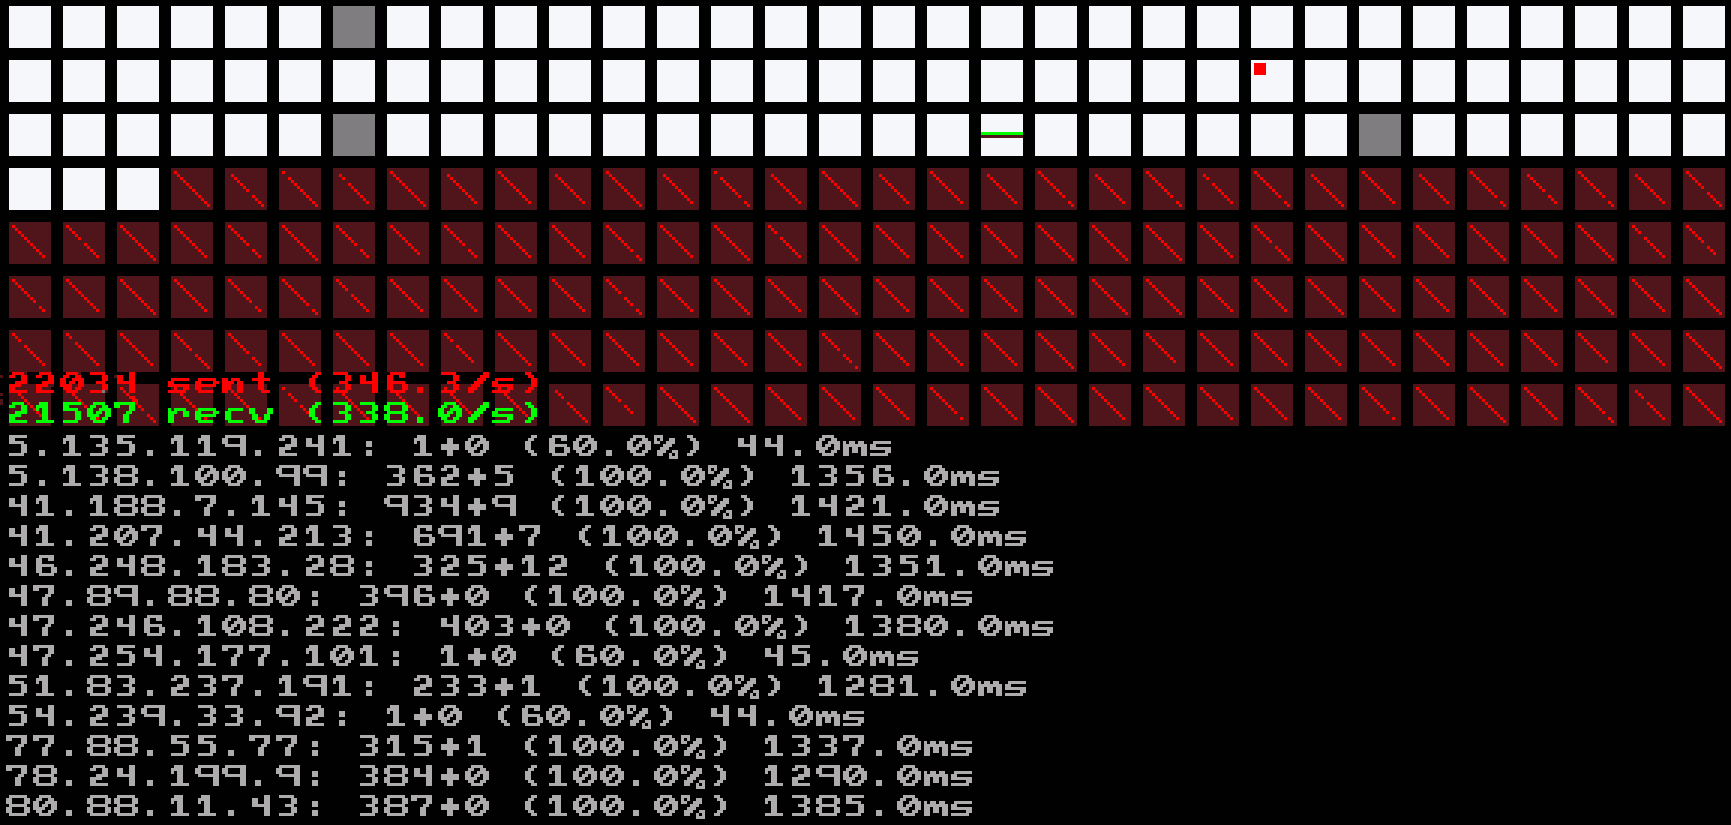
\includegraphics[width=\columnwidth]{pingu-viz}
  \caption{Visualization of the {\tt pingu} drive (truncated). The
    squares at the top are the data blocks; where white indicates
    a healthy block with a full complement of outstanding pings,
    and darker colors less so. The crossed-out blocks have not yet
    been written (and so store no data). The red dot indicates a
    block with an outstanding write, and the green bar the current
    block for the round-robin initialization. At the bottom, some
    of the hosts and their recent statistics.
  } \label{fig:pingu-viz}
\end{figure}

\subsubsection{Results}

Next we want to evaluate this Harder Drive according to various
criteria. Our goal is not to create a drive that is ``good'' according
to normal criteria like speed, but it is still interesting to benchmark
it.

For each benchmark in this paper we will store a single file on the
drive. The choice of file typically doesn't matter for the benchmark
(which will compute ``bytes per second'' etc.) but it very much
matters for the aesthetics of the project. In each case we'll choose a
file that establishes a kind of ``improper
hierarchy''~\cite{murphy2018improper}. For {\tt pingu}, we'll store
RFC 792~\cite{rfc792}, a 29,186-byte text file that describes ICMP,
including the \icmpecho\ and \icmpechoreply\ messages with which we've
constructed the drive.

Before benchmarking, we format the drive with a FAT12 filesystem and
mount it ({\tt -noatime}, etc.). We then {\tt sync} and flush the
kernel cache.\footnote{ \verb+echo 3 > /proc/sys/vm/drop_caches+ }
Flushing cache is very important, as these tiny drives easily fit
entirely within the cache and appear to be very fast if you don't do
this. Then, the benchmark writes the entire file to the test drive,
syncs and clears cache again, and reads it back, comparing to make
sure the correct bytes were written. We repeat this process over and
over, for at least one minute (though some drives will only complete a
single pass, taking much longer than a minute). The sync/flush between
writing and reading is attributed to the write time, because this is
when the writes are actually taking place.



% Results for /mnt/pingu, file rfc792.txt (29186 bytes):
% Writes: 437790 bytes in 28.64s, 15286.94 bytes/sec
%  (0 short writes)
% Read: 437790 bytes in 33.07s, 13239.73 bytes/sec
%  (0 short reads) (0 errors, accuracy: 100.000%)
% Finished 15 iters in 64.79s.
% 0.2315 iters/sec 13514.23 bytes/sec overall


% Results for /mnt/compu, file compu.cc (6835 bytes):
% Writes: 355420 bytes in 58.08s, 6119.43 bytes/sec
%  (0 short writes)
% Read: 355420 bytes in 0.04s, 10086855.31 bytes/sec
%  (0 short reads) (0 errors, accuracy: 100.000%)
% Finished 52 iters in 60.59s.
% 0.8582 iters/sec 11731.69 bytes/sec overall


\paragraph{Qualitative.} This is a good Harder Drive. It solves
a problem we don't have, which is to unreliably store a small amount
of data in an even smaller amount of memory.\!\footnote{ I considered
  whether it would be possible to create a drive that used {\em no}
  memory for each additional block, and how I might even
  define/measure that. This lead me to a brief experiment with {\tt
    compu}, which never graduated to a proper Harder Drive. This drive
  compiles the drive's contents as code, namely a large switch
  statement that is of the form \verb+case ADDRESS: return DATA;+ for
  each address in storage. The joke is of course that if you don't
  count the ``code'' towards memory, you can sneak memory into the
  code. Of course, to write to the drive, we need to rewrite the code
  and recompile it (this is done dynamically by forking \verb|g++| and
  then loading the recompiled symbol with \verb|dlopen| (which
  obviously uses memory)). I was hoping that the compiler would be
  able to do some clever optimizations on the switch statement, which
  might have led to some interesting developments. But the only ones I
  observed were the cases where the entire contents are the same byte,
  or where each address contains the low byte of the address as data.
  Otherwise it always just compiled as a table lookup, which is pretty
  uninspiring. For completeness, this drive was annoyingly fast in
  benchmarks (of course using its own source code as the benchmark
  test file): 6,119 bytes/sec writing; 10 Megabytes/sec reading. } It
treats latency as a desirable quantity, contrary to the usual
preference. Implementing the drive was much more difficult than
expected from back-of-the-envelope calculations.

\paragraph{Cost.} The cost consists of an up-front cost (a computer
and network interface; even a \$35 Raspberry Pi should work fine) and
an incremental cost per byte stored. This drive is unusual in that
storage is derived from network bandwidth, which is measured in bytes
per second. My home network is ``1 Gigabit/sec'' and \$80/month
($\$3.04 \times 10^{-5}$ / second). Storing 51,200 bytes renders the
connection otherwise unusable, so we assume this is close to the
maximum storage. This is a cost of 0.156 cents per byte per month,
which is $5.94 \times 10^{-8}$ cents, or 59.4 nanodollars, per byte
per second.

\paragraph{Longevity.} Longevity is poor. The one-minute benchmark
succeeds with 100\% accuracy, but data will readily be lost if the
drive is left running for several minutes. We can increase longevity
by using hosts with higher latency, although this reduces
speed.\!\footnote{ One easy approach is to deliberately incur
  additional overhead. For example by connecting to a VPN in Nigeria,
  I ensure a round-trip to Africa before the pings even make their way
  to the open Internet, which increases latency significantly. This
  reduces throughput to 2,948 bytes/sec., however.} Since the data are
stored externally using untrusted hosts around the world, it is easy
for adversaries to tamper with it by sending us back the wrong data.
This could be mitigated with checksums or error correcting
codes~\cite{reed1960polynomial}, although we want to avoid anything
that might resemble ``storing'' the data locally (this is cheating).
On the other hand, since we do not store data locally, this drive
could be considered ``non-volatile'' in the sense that if we
completely lose power and reboot, we can still recover the data as the
pings are received from the network. Such a reboot would need to
happen in less than about 100 milliseconds, though.

\paragraph{Speed.} The drive is slow but tolerable. In the benchmark
wrote and read the test file 15 times in one minute, and achieved
15,286 bytes/sec writing and 13,239 bytes/sec reading. Reads and
writes are basically the same operation so this gives a small
indication of the variance (high) as well. We can get better I/O
performance by using hosts with lower latency, but this increases the
(local) cost and decreases longevity.

\paragraph{Power.} Power consumption is low. The up-front power cost for
a computer and network connection is small (Raspberry Pi 3 is about
3~Watts). The data are actually stored externally, and if we were the
only use of the Internet, a very significant amount of power would be
consumed in transmission lines. In the benchmarked configuration, each
512-byte block has 4 outstanding pings, for which we assume a mean
cable length of 1/4 Earth circumference (10~Mm). A copper connector
like Cat6 UTP has nominal DC resistance of 84~$\Omega$/km, so the loop
resistance would be 840~M$\Omega$, which is actually rather high. The
math to figure out the power per byte eludes me (not to mention that
undersea cables are usually fiber optics), but it is not trivial. A
typical undersea data cable's excitation power is on the order of tens
of kilowatts, with repeaters every 100~km or so. Fortunately, the
total bandwidth of such cables is extremely high, with these 512-byte
packets representing a minuscule fraction. Rather than try to multiply
a big estimate by a small estimate, it is better to work from a known
quantity: Assuming that the cost of the consumer internet connection
also covers the marginal cost of the power in these backbones, at
$0.15c/kwH$, this seems to be at most 5.8~$\mu$Watts per byte-second.

% Not sure this makes any sense?
% 0.15 * 125,000,000 bytes / 0.0000304 * (1000 * W) * 60 * 60 * sec)
% 18750000 bytes / 109 Watt * sec
% (125,000,000 bytes) / $0.0000304

\paragraph{Is rotational?} One of our criteria will be whether the
drive should set the \verb+is_rotational+ flag for {\tt nbdkit}
(Section~\ref{sec:nbdkit}). The inspiration for this drive (orbital
chainsaws or radio towers around the world) would be rotational, but
this drive is not. Although the initialization happens round-robin,
due to the stochastic timing of the outstanding pings, the drive soon
thereafter processes the blocks in a random order.

\paragraph{Harm to society.} The drive is definitely harmful to my
home network; whether that can be considered a positive or negative to
society is left as an exercise for the reader. At the benchmark scale
of 51,200 bytes, the effect on the broader internet is trivial, and I
took care to not overwhelm any particular host. However, at scale
this drive would be harmful to the shared infrastructure, and
carries the moral hazard of ``freeloading'' off the willingness of
hosts to reply to \icmpecho\ messages.
% internet peering relationships

\section{Tetris, the Soviet Mind Game} \label{sec:tetris}

Sorry to remind you about Vladimir Putin's illegal invasion of
Ukraine, but this section concerns a hard drive made from the best
Russian (actually, Soviet) video game, Tetris~\cite{pajitnov1984tetris}.

Tetris is an inventory-management survival-horror game with 19
principal characters, each with its own story arc; they are: 
\ivert
\ihoriz
\squarepiece
\tup
\tdown
\tleft
\tright
\jup
\jleft
\jdown
\jright
\zhoriz
\zvert
\shoriz
\svert
\lup
\lleft
\ldown
\lright

Like all living things, these characters are made up of four
individual pixels, or ``blocks.'' By being confused about the fact
that words can have multiple meanings, we can have an idea: Make a
block device from these blocks, using their presence or absence in the
playfield to store data. A Tetris board is 10 columns wide and 20 rows
high. Even if we could use every one to store a bit, 200 bits is far
too few to create a filesystem. Therefore we'll use an array (or if
you will, a {\em Beowulf cluster}) of Tetris games to create the block
device.

We will store a bit pattern in a Tetris game by playing a series of
moves to create a specific pattern in the playfield. We can then read
the data directly from that pattern. If we need to write a new
pattern, we reset the game and begin again.

Each ``line'' of the playfield has 10 positions, each of which could
have a block in it or not, so we could consider storing 10 bits.
However, due to the rules of Tetris, if all of the cells are filled,
then the line is cleared. This would make it impossible to store the
pattern {\tt 1111111111}. It will also be impossible to store the
pattern {\tt 0000000000}, because an empty line cannot support any
pieces above it, so empty lines can only appear in some
completely-empty prefix of the playfield. Additionally, observe that a
Tetris board always has an even number of cells filled. We can only
add 4 blocks by dropping a piece, or remove 10 blocks by clearing a
line, which can only yield even numbers. So it will also benefit us to
have one free cell per line for parity. A good choice is to use 8
cells per line for data, encoding a single byte, which is a nice round
number.

We can't use the full height of the playfield, since we need some room
in which to maneuver pieces. 8 is a convenient choice here as well
(although more is possible). Each Tetris game will thus store 64 bits:
Eight lines, each with eight bits. We'll use the venerable NES Tetris
(Nintendo, 1989), which is also 8 bits.

% I tested 10 bits; 529 examples successful. 12 fails, though (would
% perhaps need to plan inside a more cramped space? or is the game
% just getting too fast and we can't force RNG?)

\subsection{Playing Tetris}

Now the problem is: Given a blank board, what sequence of moves do
we make in order to produce the target pattern?

This is not easy. To begin with, Tetris normally gives the player
pieces at random. As anyone who plays Tetris knows, it can be very
disruptive to your strategy when you don't get the piece you need for
some time. The first step will be to reverse engineer the pseudorandom
piece drop logic so that we can influence the sequence of pieces that
are dropped.

\subsubsection{Random pieces}

The core of the piece drop logic is a 16-bit linear feedback shift
register~\cite{golomb1967shift}.\!\footnote{Fittingly, Golomb was a
  pioneer in both shift registers {\em and} polyominoes, the latter
  which influenced Tetris itself!} Equivalent C code is given in
Figure~\ref{fig:nextrng}. This 16-bit state is updated on every frame
(and sometimes more; see below), and has period 32767.\footnote{ It is
  possible to create a 16-bit LFSR with a period of 65535, but this
  one is simply deficient. This is one of several small problems with
  the code. I hope to one day release a ``hot fix'' ROM that fixes
  this and other bugs and inefficiencies.}

\begin{figure}
  \centering
  \begin{lstlisting}[language=C]
uint16_t NextRNG(uint16_t state) {
  uint16_t carry = ((state >> 9) ^ (state >> 1)) & 1;
  return (state >> 1) | (carry << 15);
}
  \end{lstlisting}
  \caption { The simplified code for NES Tetris's pseudorandom number
    generator, which resides at address {\tt 0xAB47} in the Tetris
    code. This is a 16-bit two-tap LFSR: The {\tt carry} is the
    exclusive-or of the second and tenth least significant bits. We
    right-shift off the least significant bit and use the carry as the
    new most-significant bit.} \label{fig:nextrng}
\end{figure}

The pseudorandom state is extended with two additional bytes: One
giving the last dropped piece (a piece is ``dropped'' into a queue so
this is actually the ``next piece'' to the player) and the count of
pieces dropped (mod 256). When the player places a piece, the routine
at address {\tt 0x9907} uses the LFSR state and these two bytes to
drop a new piece (and update the state):

\begin{lstlisting}[language=C]
RNGState NextPiece(RNGState s) {
  constexpr std::array<uint8_t, 8> PIECES = {
    0x02, 0x07, 0x08, 0x0A, 0x0B, 0x0E, 0x12,
    /* not used */ 0x02,
  };

  s.drop_count++;

  uint8_t a = (s.lfsr_hi + s.drop_count) & 7;

  if (a == 7 || PIECES[a] == s.last_drop) {
    // re-roll if out of bounds, or repeat
    s = NextRNG(s);
    // mod 7 forces in-bounds, but allows repeats
    a = ((s.lfsr_hi & 7) + s.last_drop) % 7;
  }
  
  s.last_drop = PIECES[a];
  return s;
}
\end{lstlisting}

It uses three bits of the RNG state to pick a random piece (there are
7 different shapes, and the game always drops a shape in the same
orientation). If it rolls an 8, or if the selected piece is the same
as the last one, then it re-rolls: Another update of the LFSR, and
then a different weird procedure to pick the piece index. Here the
result is {\sf mod}~7, so it is always in bounds. The code only
re-rolls once, so it is possible to drop the same piece twice in
a row, just less unlikely.

Ideally we would be able to select a sequence of pieces that we want,
and then force Tetris to give us those pieces. Since the LFSR update
runs every frame, we can use a different number of frames while
placing a piece, and get a different LFSR state at the point {\tt
  NextPiece} is called. The LFSR is ``pretty good,'' so we can easily
cause the first roll to be whatever value we want by just waiting. In
the worst possible case we need to pause 98 additional frames before
seeing all 8 rolls (Figure~\ref{fig:rollhisto}), which is 1.6 seconds
at the NES frame rate.

However, this does not work for re-rolls, which is the only way to get
the same piece twice in a row. Even though we use the same ``pretty
good'' LFSR to get the second pseudorandom number, two successive
calls are highly correlated. There are only two possible new values
for the high byte of the LFSR (\verb|s.lfsr_hi|):
\verb|(s.lfsr_hi >> 1)| and \verb|128 + (s.lfsr_hi >> 1)|. Worse,
since these are congruent modulo $8$, we really just have
\verb|(s.lfsr_hi >> 1)|.
 
As a result, even if you have complete control over the LFSR state
(but not the previous piece nor drop count), there are a limited
number of outcomes possible from the reroll. We can just inspect all
the possible combinations of previous piece and drop count to see that
with some there are at most 4 possible rerolls, and as few as 2. For
example, if the previous piece is \shoriz\ and 253 pieces have been
dropped so far, then only \tup, \shoriz, and \jdown\ can result. So
here it is possible to get two \shoriz\ pieces in a row. But if the
last piece was \ihoriz, and 3 pieces have been dropped so far, then
only \zhoriz\ and \lup\ are possible from a re-roll. Since
\ihoriz\ cannot result from the first roll and is not possible for the
re-roll in this state, it is impossible to get two \ihoriz\ pieces in
a row on the 3\rd\ and 4\th\ drop. All pieces other than
\squarepiece\ periodically have this problem.\!\footnote{This is
  another example of a deficiency in the code that could easily be
  fixed. If we simply remove the instruction at {\tt 0x9925},
  \verb+AND #$07+ (so that the re-roll just uses
  \verb|(s.lfsr_hi + s.last_drop) % 7|) then {\it all} configurations
  can now produce all pieces upon re-roll. The modulus is computed
  with a loop, so this is not a strict efficiency improvement, but
  efficient alternatives with this property exist,
  like \verb|((s.rng2 & 15) ^ s.last_drop) % 7|.
} Even when it is possible, it may
require a long drought to get the LFSR in a rare working state.

\begin{figure}[ht]
  \centering
  \includegraphics[width=\linewidth]{rollhisto}
  \caption {
    The maximum possible ``drought'' for the NES Tetris LFSR. This is
    the number of iterations before we see all possible rolls (all
    eight possible values for the low three bits), histogrammed
    over all meaningful start states (LFSR state and drop count).
    The minimal value is 8 (obviously, by pigeonhole) and rarely
    it can be as high as 99, but most of the time we have seen
    all rolls by a few dozen iterations.
    } \label{fig:rollhisto}
\end{figure}

By manipulating the RNG we will be able to achieve any sequence of
pieces, except if that sequence contains repeats. There is a similar
consideration for the first two pieces of the game, which are
generated on the same frame (current and next piece) and so only
certain combinations are possible. To simplify this issue away, we
begin by always playing the same starting sequence: \squarepiece 0
\lleft 3 \jright 6 \lright 2 \jleft 7. This means to drop a
\squarepiece\ in column 0 (the leftmost column), \lleft\ in column 3
(the left edge of the piece goes in column 3), etc. This sequence
clears two lines, leaving the board empty, with the only constraint
now being that we cannot start with a \jleft\ piece. In fact we will
always start with a \svert\ piece in the leftmost column to make
use of the modular plans described in the next section.

\subsubsection{Planning}

With a smart algorithm, it would be possible to plan moves within
these constraints to generate moves for any byte pattern that we want
to create. However, this is not an easy feat. Creating very sparse
patterns (few {\tt 1} bits) is pretty challenging because pieces can
only be placed on top of existing blocks (Figure~\ref{fig:tetrisdot}).

\begin{figure}
  \centering
  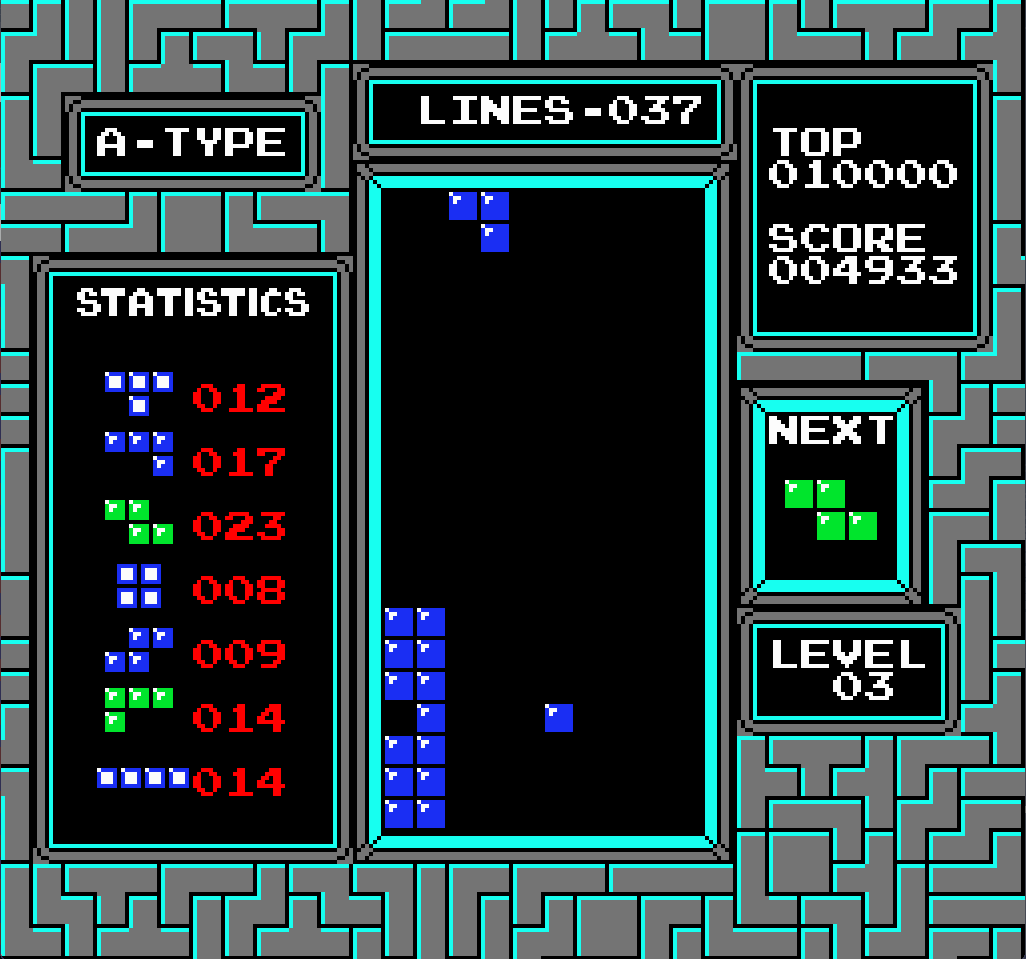
\includegraphics[width=\linewidth]{tetrisdot}
  \caption{
    A screenshot of NES Tetris after playing for 2 minutes and 46
    seconds, encoding the sequence {\tt 0, 0, 0, 0, 64, 0, 0, 0}.
    Floating blocks like this are very difficult to make. Try
    creating a position like this, even by selecting your favorite
    piece at each step!
  } \label{fig:tetrisdot}
\end{figure}

Instead, the approach I took was to build a modular solution for each
byte. We always place the board in a standard configuration
(Figure~\ref{fig:encodingscheme}) where a \svert\ piece is in column
0. A portion of the board below it contains the encoded bytes (one per
row) and parity (first two columns). We do not depend on the contents
of this portion at all, so the first moves must hang off of the
\svert\ piece. For each byte, we need to come up with a series of
moves that takes a starting configuration like this, encodes the byte
(and its parity) in the bottom row, and then recreates the starting
configuration with the \svert\ piece moved up one line. These plans
are also nontrivial to construct, but we can take our time to solve
each byte offline. Then, because they are compositional, we can assemble
them to create any sequence of bytes at runtime.\footnote{
  As one final complication, when we concatenate two of these sequences
  we still need to avoid repeat pieces. We do this by only allowing a
  sequence to end with the \shoriz\ or \ihoriz\ pieces, and not
  allowing either of those to start sequences.}

\begin{figure}
  \centering
  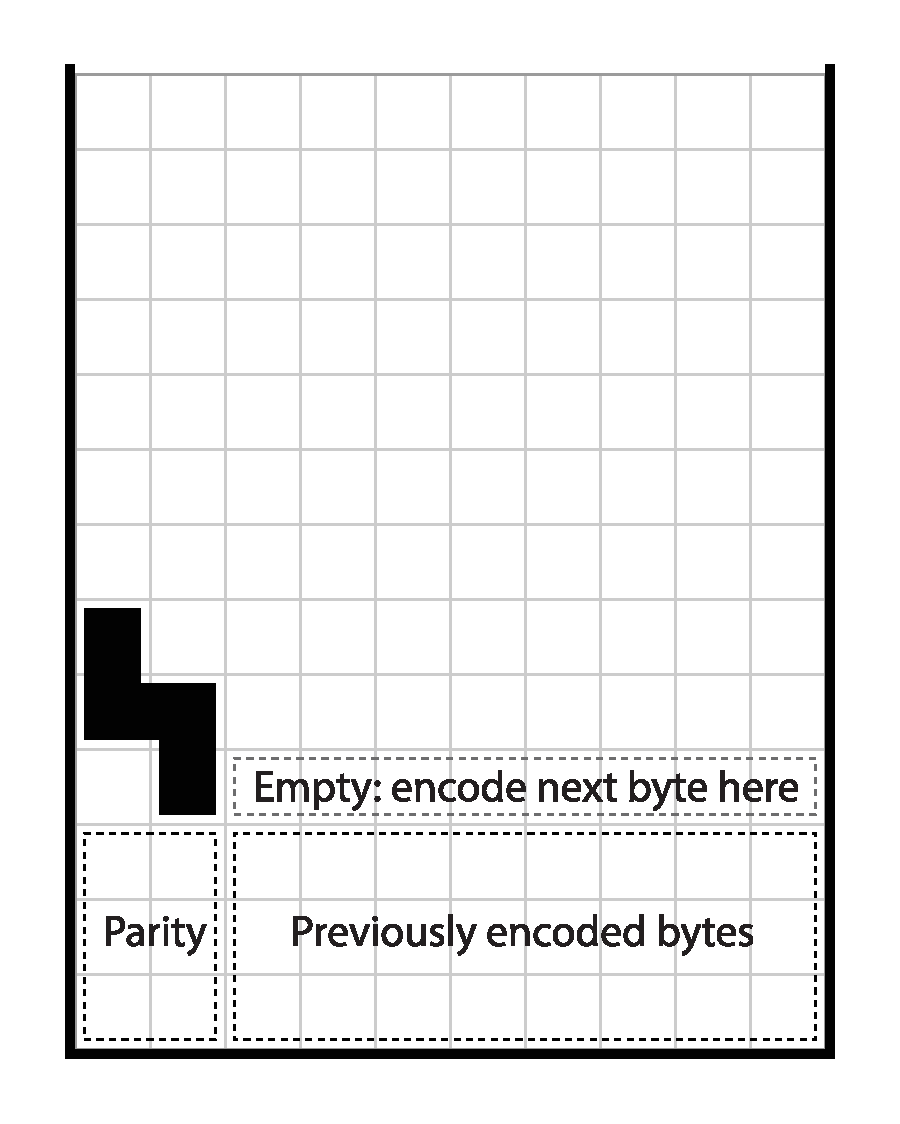
\includegraphics[width=0.6 \linewidth]{encodingscheme}
  \caption{
    The start state as we encode each byte. The \svert\ piece in the
    left column is known to be present, but we do not know the state
    of any blocks below it. We will only build off of this block so
    that the solution works regardless of what is below, and at
    any height (as long as there is enough headroom in the playfield).
    The parity columns will be {\tt 0b01} or {\tt 0b11} as appropriate,
    except in the case of the byte {\tt 0xFF} we use {\tt 0b00} so that
    we don't create and clear a line.
    A specific example solution is given in Figure~\ref{fig:encode26}.
    } \label{fig:encodingscheme}
\end{figure}

\begin{figure}
  \centering
  \begin{tabular}{cc}
  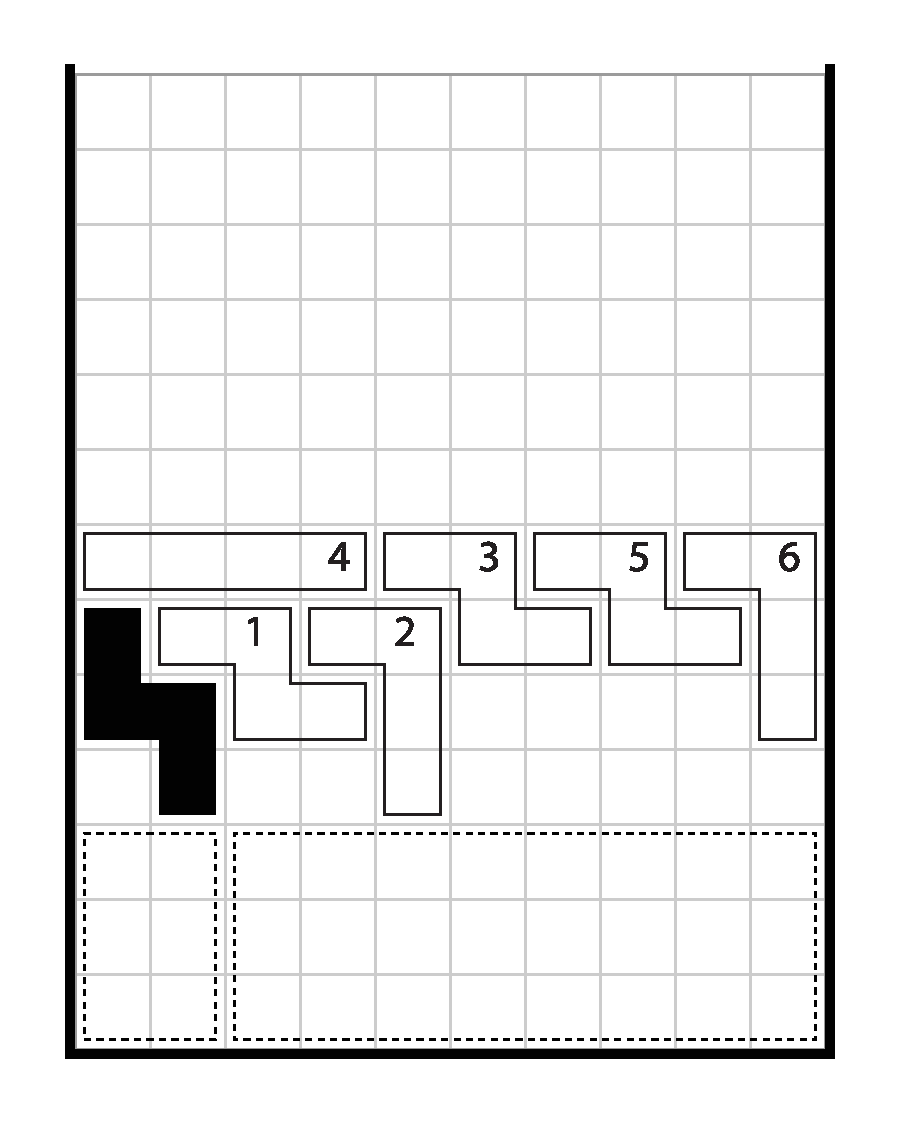
\includegraphics[width=0.4 \linewidth]{encode26a} &
  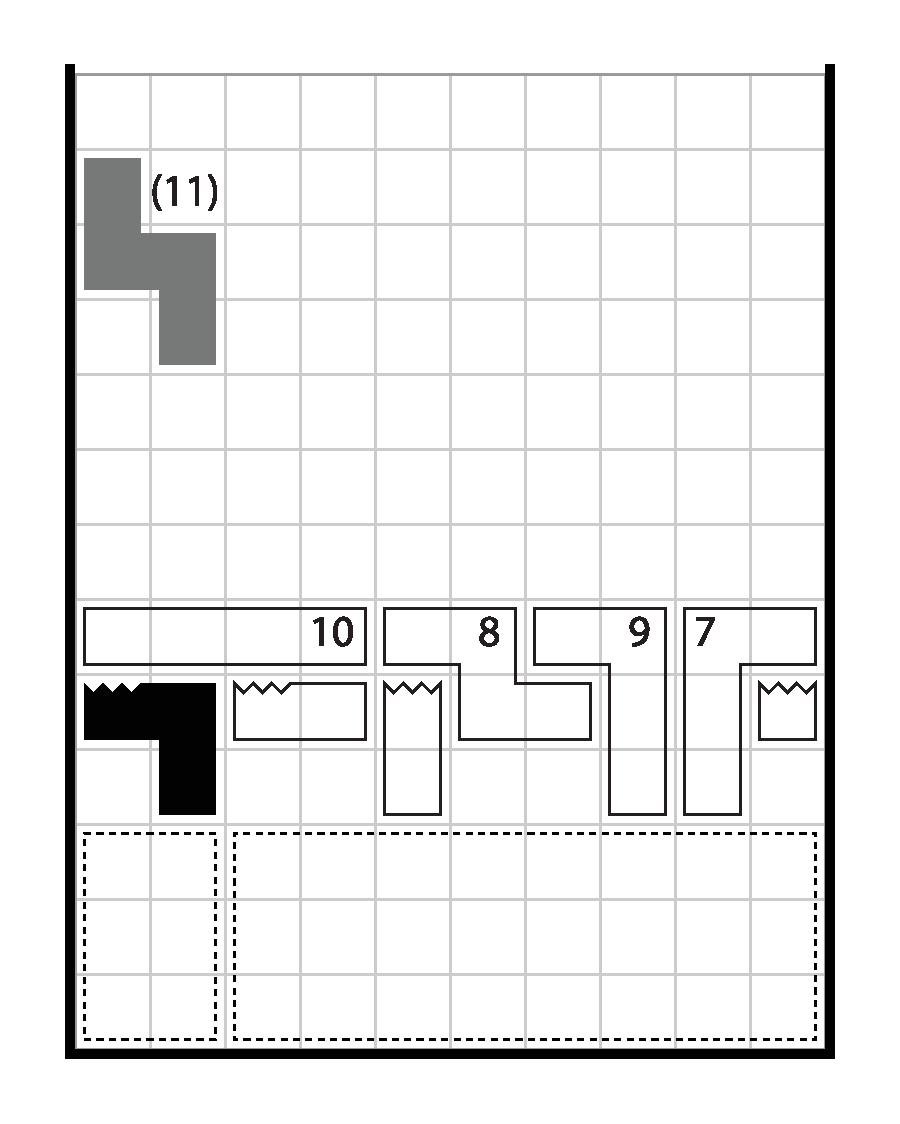
\includegraphics[width=0.4 \linewidth]{encode26b} \\
  (a) & (b)
  \end{tabular}
  \caption{ Encoding {\tt 0x26}, which is {\tt 0b00100110}. This is one
    of the easiest bytes. In (a), drops 1--6 build off of the starting
    \svert, conveniently dropping a {\tt 1} bit in column 4 along the
    way. These moves clear the two top lines, leaving some partial
    blocks. Note that we use \zhoriz\ and \ldown\ multiple times, but
    never consecutively. In (b) we use some of the floating pieces to
    fill the remaining {\tt 1} bits, clean up by making two more
    lines, and then drop a \svert\ onto known support in order to put
    ourselves back in standard position, one line higher. Many
    sequences create the ``\svert'' shape through means other than
    placing it literally. } \label{fig:encode26}
\end{figure}

An example sequence is illustrated in Figure~\ref{fig:encode26}. They
are not easy to construct by hand, but it is not too hard to find them
with computer search. I have a two-phase heuristic search: First,
a heuristic that measures how close we are to placing the correct bit
pattern in the bottom row (with penalties for covering bits that we
still need to set, or for growing the pile too high). Second, measuring
how close we are to reaching the standard start position (by clearing
any leftover stuff).\!\footnote{Details here are in {\tt encode.cc}.
  My first attempt worked pretty well, so I didn't fiddle with it
  much; no doubt it can be improved!} This finds solutions for all
bytes easily; to find really good short sequences we just run it for
hundreds of hours. This search uses my own implementation of Tetris,
which can be simplified because e.g.~we only drop pieces straight down.
It is orders of magnitude faster than emulating the NES Tetris ROM.

With this setup, the best solutions I know of for each byte (as of
publication) are as follows:

\begin{figure}[ht]
  \centering
  \includegraphics[width=1.66in]{hyrule}
  \caption{
    The number of Tetris pieces placed to create each byte, with
    light being the fewest (11) and dark being the most (22). The
    first row is ({\tt 0x00}, {\tt 0x01}, \ldots). We tend to need
    fewer moves to create bytes with fewer {\tt 1} bits, and there
    are some symmetries and patterns visible. On the other hand,
    I was somewhat disappointed not to see the familiar Triforce
    pattern appear here, as it has so many times before~\cite{murphy2014new,murphy2017zm,murphy2018making}. It may be that these solutions are not yet
    optimal (but they are probably close). Alternatively, 
    it could be that this is the {\em exception that proves
    the Hyrule.}
  } \label{fig:hyrule}
\end{figure}

% FIXME re-enable
\input{solutions}

An earlier version of this table did not fit neatly into the column.
Rather than fiddle with \LaTeX\ layout, I instead expended significant
CPU time to further optimize the problematic rows until they would
be short enough to fit! This is the {\em true spirit of typography}.

\subsubsection{Executing}

Now that we have a solution for each byte, we want to play the NES
game to put the desired pattern in the playfield. We use a NES
emulator (my version of FCEUX~\cite{fceux} which I've heavily modified
for e.g.~thread-safety) which allows us to save and restore states,
inspect RAM, and execute frames much faster than real time.

We always input a fixed sequence of button presses to the emulator to
begin a game with the right starting pieces. We then start executing
the plan, which consists of the fixed starting sequence (puts us in an
empty board with \svert\ in the leftmost column) and then the
concatenation of the plans for the bytes we want to encode. All that
is left is to place pieces according to this plan, while ensuring that
we get the desired sequence of ``random'' piece drops.

At the start of each piece, we save the emulator state, and then
navigate the piece into the correct column. Holding down on the D-pad
causes the piece to drop as fast as possible. When it lands, if we got
the correct piece by chance, we just continue. Otherwise, we inspect
the state of the random number generator (right {\em before} the piece
dropped), and then simulate it using our reverse engineered version.
We tabulate the piece that would drop if we were to take one
additional frame to get here, then two, then three, and so on up to
some fixed horizon.\footnote{The longest possible drought before we
  see the desired piece (if we missed it on the first attempt) is 98
  frames (Figure~\ref{fig:rollhisto}). But it is helpful to build in
  significant redundancy, since there are some unusual situations
  where we cannot drop exactly on a desired frame, and must
  overshoot.} We can then restore the saved state and drop the piece
more slowly (not pressing down on the controller), delaying for the
correct number of frames to get the piece that we want. We can usually
get this exactly right on the first try, but if not, we try again with
slightly longer or shorter delays until successful. It is also
possible to pause the game~\cite{murphy2013first} if the delay needs
to be longer than the natural descent of the piece, which can happen
when the game speeds up at later levels and the pile is high.

\subsection{Harder Drive: Tetru}

We can now build a hard drive with Tetris. It's called {\tt tetru},
following the convention from Section~\ref{sec:pingu}.\footnote{Also
  because Tetris is Russian and {\tt .ru} is the TLD for Russia.
  Classic retcon which I just nailed.} The setup is straightforward:
The block size is 8 bytes, and each block consists of a NES Tetris
emulator. When we first write a block, we allocate the emulator, load
the Tetris ROM, and use the procedure above to supply inputs to the
game. The driver is multithreaded so 16 concurrent Tetris games can be
in progress, although the block size is so small that we need several
serial passes to write one ``normal'' 512-byte sector. To read a
block, we just inspect the 200 bytes of memory at {\tt 0x400}.
The byte {\tt 0xEF} is an empty cell ({\tt 0}) and any other byte is some
part of a tetromino ({\tt 1}).

If we re-write a cell, we reset the emulator and start again. It might
be possible to clear the playfield by playing the game (for example it
would be straightforward to precompute a plan that clears any bit
pattern on a single line, parity issues notwithstanding). But as the
game gets faster and faster we may be unable to drop pieces in the
correct locations, so it is safer to reset. This is something the
player can do anyway, so there is no loss of authenticity.

Finally, as an optimization, we also cache the input sequence that we
compute for the 8 bytes the first time we do it; if we write that same
pattern again then we can just replay the inputs rather than search
for them a second time. Both the FAT12 directory structure and benchmark
file have many repeated patterns (especially $8 \times {\tt 0x00}$),
giving us a good cache hit rate of 46\% during benchmarking.

Of course, there would be other ways to make this faster, too. For
example, just the pointer to the emulator object for each block is 64
bits, or 8 bytes itself, suggesting a form of ``content-addressed
storage.''

\subsubsection{Results}

In order to benchmark we need some file to write to the filesystem. A
beautiful choice is the {\tt tetris.nes} ROM file, which is 49,168
bytes. Though the minimal filesystem for FAT12 requires a device with
51,200 bytes, there is significant overhead from the filesystem
header, directory entry, and so on. So to store this ROM we create a
device with 69,120 bytes, which is 8,640 NES emulators. It is
straightforward to scale to thousands of emulators, with the biggest
challenge being to fit them all on the screen for some kind of
visualization.

\begin{figure}
  \centering
  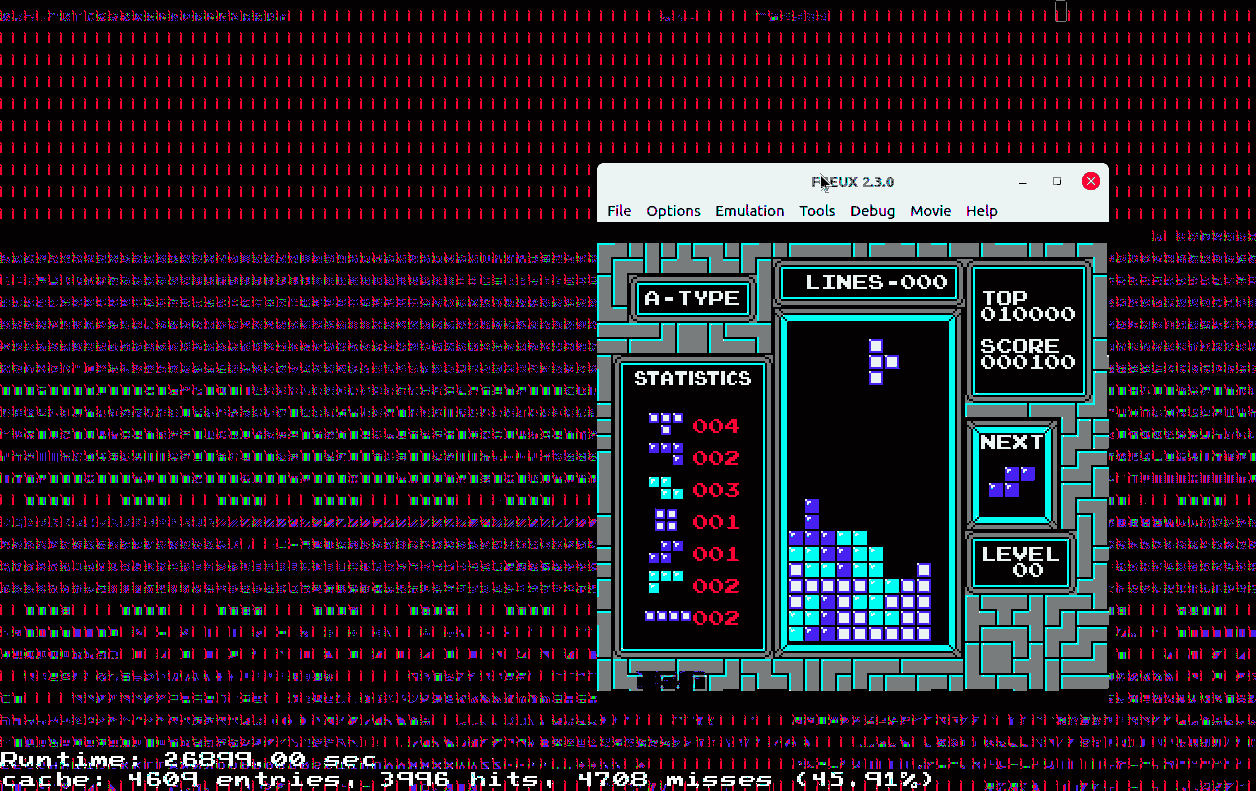
\includegraphics[width=\columnwidth]{tetru-playing}
  \caption{ Playing a game of Tetris in the FCEUX emulator, in which
    we loaded the {\tt tetris.nes} ROM from the {\tt tetru} drive. The
    backdrop is a truncated portion of the visualization showing the
    contents of the 8,640 Tetris boards being emulated. The upper
    portion is the FAT-12 header and directory entries (it is mostly
    {\tt 0x00}) and the lower portion is the ROM data. I only have 100
    points right now but as you can see I am gearing up to complete
    some sweet, high-scoring Tetrises. } \label{fig:tetru-playing}
\end{figure}

We benchmark as before, but then of course it is important for
aesthetic reasons to load the ROM that we stored inside the drive
to play a game of Tetris. Figure~\ref{fig:tetru-playing} shows
this in practice.

\paragraph{Qualitative.} This is a good Harder Drive. It solves a problem
we don't have, which is that typical hard drive ``blocks'' are not made
of actual ``blocks,'' but Tetris players will recognize that the data on
the drive is indeed made from blocks. It is very satisfying to watch
the thousands of Tetris games drop pieces to encode the data.

\paragraph{Cost.} Simulated on a computer, the up-front cost of storing
data is fairly low. A basic 16-core desktop computer is about \$1,800
in 2022. The software NES emulator uses 1,652,372 bytes of RAM for
Tetris on a 64-bit machine, which is 650 instances per gigabyte. So we
can store about 5200 bytes in about \$4.37 worth of RAM,\footnote{ In
  2022, a Corsair 16GB DDR4 DIMM is only \$70. } which is 0.084 cents
per byte. This could easily be improved; the emulators could be stored
much more efficiently, because they are all emulating the same ROM. If
we built this with actual Nintendo hardware, we would need one NES
Console and one Tetris cartridge (or bootleg) per eight bytes. A used
NES runs about \$150 and a Tetris cartridge about \$10. This is
\$20 per byte, which 24 thousand times more expensive.

\paragraph{Longevity.} The stored data lasts indefinitely, as long as
the computer (or Beowulf cluster of NES consoles) remains powered.

\paragraph{Speed.} Writing the 49,168-byte test file {\tt tetris.nes}
takes 3 hours, 18 minutes and 52 seconds, for a data rate of 2.57
bytes/sec. Due to its caching nature, writing to the hard drive gets
faster as it stores more data. Reading is much faster at 61,430 bytes/sec.

% runtime 26899 sec
% 4609 cache entries, 3996 hits, 4708 misses, 45.91%
% 
% Results for /mnt/tetru, file tetris/tetris.nes (49168 bytes):
% Writes: 49168 bytes in 19132.53s, 2.57 bytes/sec
%  (0 short writes)
% Read: 49168 bytes in 0.80s, 61430.56 bytes/sec
%  (0 short reads) (0 errors, accuracy: 100.000%)
% Finished 1 iters in 19133.49s.
% 0.0001 iters/sec 5.14 bytes/sec overall
% 
% real	318m54.336s
% user	0m0.015s
% sys	0m0.687s


\paragraph{Power.} On a modern computer, a gigabyte of RAM uses about
375~mW of power~\cite{crucialpower}, so the marginal cost is 72~$\mu$W
per byte. The NES console uses about 10 Watts, which would give us
about 1.25~W per byte.

\paragraph{Is rotational?} This drive \verb+is_rotational+, because the
Tetris pieces are rotated to place them in the correct orientation.

\paragraph{Harm to society.} There is no harm to society for the software
emulation. If built on real NES consoles, hoarding thousands of these
machines and cartridges would be considered antisocial, as they are
historic items that are in limited supply, and many people still enjoy
collecting and using them for their intended purpose.


\section{Cue the coronavirus} \label{sec:cue}

Speaking of using things for their intended purpose:
Sorry to remind you about the worldwide pandemic still killing
thousands of people every day, but this section concerns a hard drive
made from COVID-19 tests.

SARS-CoV-2 is an RNA coronavirus first isolated in January
2020~\cite{wu2020coronavirus}. Since it is highly contagious and can
cause severe illness (especially in the immune-na\"ive), testing is an
important part of the worldwide response. There are two widely
available approaches to testing: Lateral flow antigen tests and PCR.
Lateral flow tests detect a target molecule (e.g.~the SARS-CoV-2 spike
protein) by binding a tagged complementary molecule (antibody) to it
as the sample flows along a capillary bed. This is awesome. The tests
are fast and cheap. Polymerase Chain Reaction
(PCR)~\cite{saiki1985enzymatic} tests work by amplifying a target
sequence of DNA exponentially. It heats and cools the sample in the
presence of a heat-stable DNA polymerase (typically {\it Taq}
polymerase, which was isolated from the thermophilic {\it Thermus
  aquaticus} bacterium) and a bubble-bath of nucleotides that can be
used to create more DNA. Each thermal cycle first unzips a
double-stranded molecule into two pieces, and then reassembles each
one, doubling the target. Properly, the tests are reverse
transcription PCR~\cite{bustin2000absolute}, because first we need to
turn the viral RNA into DNA. PCR tests are more sensitive (they can
detect a {\em single} molecule) and specific (they detect a particular
genetic sequence). This is also awesome.

{\it Cue} is a bougie COVID-19 test that launched in 2021. The test
consists of a reusable reader (\$200) and a single-use cartridge (\$65
{\em each}!). Notwithstanding the eye-popping expense, the system is
pretty good. My employer provides these tests for free (!), so I
started collecting the used cartridges over the course of several
months, and soliciting them from my friends as well.

The cartridge itself (Figure~\ref{fig:cuetechnical}) is fairly
ingenious and deserves to be disassembled.\footnote{I recommend only
  disassembling a ``negative'' test, in case that is not obvious. The
  typical reagents used in RT-LAMP are not particularly dangerous; for
  example
  % JK if it is isothermal, like LAMP, then this is perhaps {\it Bst}
  % polymerase: Bacillus stearothermophilus
  %
  % https://www.neb.com/products/m0275-bst-dna-polymerase-large-fragment#Quality,%20Safety%20&%20Legal_Safety%20Data%20Sheets
  % {\it Taq} polymerase is ``not hazardous'' according to OSHA,
  {\it Bst} polymerase is ``not hazardous'' according to OSHA,
  although it may be an ``eye irritant''~\cite{neb2019bst}.} When you
stick the nose swab into the cartridge, it of course is delivering the
snotty sample, but the insertion force also mechanically actuates a
number of plastic thorns which pierce foil seals on reagent ampules,
allowing them to start their thing. The assay is described as
``nucleotide amplification,'' which would suggest something like
RT-PCR, but since the cartridge does not significantly change
temperature during a test, it is probably not literally PCR.
LAMP~\cite{notomi2000loop} is a similar technique which is {\em
  isothermal} and seems like a credible choice. Again it would be
preceded by a reverse transcription step to turn RNA into DNA. These
things are all awesome and deserve to be learned about; for example
did you know that the most frequently used reverse transcriptases
(which turns RNA into DNA to begin amplification) were isolated from
RNA viruses (which those sneaky bastards use to turn their own RNA
into DNA so that it can be transcribed by the host)? So now we're
using virus machinery to detect and fight other viruses? Hell yeah we
are!

If you pull off all the chemistry pieces from the cartridge's
endoskeleton, you'll also find a tiny 8-pin microchip onboard. And if
you have a microscope you can read that it says ST 24C04WP, which is a
serial EEPROM~\cite{stm24c0w}. An EEPROM is a programmable ROM (so it
is ``read-only'' but also writable?). It is probably used to store the
cartridge's serial number, expiration, what kind of test it is, and
maybe calibration data. This stuff would be pretty small, so it's no
surprise that the chip can only store 512 bytes. A dump of one of
these ROMs is in Figure~\ref{fig:romdump}.

% \begin{figure}
% \begin{lstlisting}[basicstyle=\tiny]
% 00 00 b6 98 d0 19 5a 45 3b ef a1 d1 41 37 e6 ec | ......ZE;...A7..
% 49 91 6f 3b ab 7d 59 32 8f d4 e1 a6 33 bf 66 4b | I.o;.}Y2....3.fK
% d6 fb 6a 9d f6 d4 89 72 a4 3d 8a 5b 62 10 4b 07 | ..j....r.=.[b.K.
% d4 c3 15 52 01 d9 20 c1 97 87 4d c2 34 df 2a af | ...R.. ...M.4.*.
% cc 05 01 00 00 00 2e 00 0a 19 08 c6 ad d6 40 10 | ..............@.
% 13 20 a3 82 01 30 80 d6 89 99 06 3a 06 32 30 39 | . ...0.....:.209
% 34 35 48 12 11 9a 01 0e 08 02 15 00 80 88 c5 20 | 45H............
% 01 2d 00 00 c8 c3 ff ff ff ff ff ff ff ff ff ff | .-..............
% 00 00 00 00 00 00 00 00 00 00 00 00 00 00 00 00 | ................
% 00 00 00 00 00 00 00 00 00 00 00 00 00 00 00 00 | ................
% 00 00 00 00 00 00 00 00 00 00 00 00 00 00 00 00 | ................
% 00 00 00 00 00 00 00 00 00 00 00 00 00 00 00 00 | ................
% 00 00 00 00 00 00 00 00 00 00 00 00 00 00 00 00 | ................
% 00 00 00 00 00 00 00 00 00 00 00 00 00 00 00 00 | ................
% 00 00 00 00 00 00 00 00 00 00 00 00 00 00 00 00 | ................
% 00 00 00 00 00 00 00 00 00 00 00 00 00 00 00 00 | ................
% 00 00 00 00 00 00 00 00 00 00 00 00 00 00 00 00 | ................
% 00 00 00 00 00 00 00 00 00 00 00 00 00 00 00 00 | ................
% 00 00 00 00 00 00 00 00 00 00 00 00 00 00 00 00 | ................
% 00 00 00 00 00 00 00 00 00 00 00 00 00 00 00 00 | ................
% 00 00 00 00 00 00 00 00 00 00 00 00 00 00 00 00 | ................
% 00 00 00 00 00 00 00 00 00 00 00 00 00 00 00 00 | ................
% 00 00 00 00 00 00 00 00 00 00 00 00 00 00 00 00 | ................
% 00 00 00 00 00 00 00 00 00 00 00 00 00 00 00 00 | ................
% 00 00 00 00 00 00 00 00 00 00 00 00 00 00 00 00 | ................
% 00 00 00 00 00 00 00 00 00 00 00 00 00 00 00 00 | ................
% 00 00 00 00 00 00 00 00 00 00 00 00 00 00 00 00 | ................
% 00 00 00 00 00 00 00 00 00 00 00 00 00 00 00 00 | ................
% 00 00 00 00 00 00 00 00 00 00 00 00 00 00 00 00 | ................
% 00 00 00 00 00 00 00 00 00 00 00 00 00 00 00 00 | ................
% 00 00 00 00 00 00 00 00 00 00 00 00 00 00 00 00 | ................
% 00 00 00 00 00 00 00 00 00 00 00 00 00 00 00 00 | ................
% \end{lstlisting}
% \end{figure}

% I <\,3 LaTeX
\begin{figure}
  \centering
{\scriptsize \tt
\noindent
  00\hspace{0.3em}00\hspace{0.3em}b6\hspace{0.3em}98\hspace{0.3em}d0\hspace{0.3em}19\hspace{0.3em}5a\hspace{0.3em}45\hspace{0.3em}3b\hspace{0.3em}ef\hspace{0.3em}a1\hspace{0.3em}d1\hspace{0.3em}41\hspace{0.3em}37\hspace{0.3em}e6\hspace{0.3em}ec\hspace{0.3em}|\hspace{0.3em}......ZE;...A7..\\[-0.25em]
49\hspace{0.3em}91\hspace{0.3em}6f\hspace{0.3em}3b\hspace{0.3em}ab\hspace{0.3em}7d\hspace{0.3em}59\hspace{0.3em}32\hspace{0.3em}8f\hspace{0.3em}d4\hspace{0.3em}e1\hspace{0.3em}a6\hspace{0.3em}33\hspace{0.3em}bf\hspace{0.3em}66\hspace{0.3em}4b\hspace{0.3em}|\hspace{0.3em}I.o;.\verb+}+Y2....3.fK\\[-0.25em]
d6\hspace{0.3em}fb\hspace{0.3em}6a\hspace{0.3em}9d\hspace{0.3em}f6\hspace{0.3em}d4\hspace{0.3em}89\hspace{0.3em}72\hspace{0.3em}a4\hspace{0.3em}3d\hspace{0.3em}8a\hspace{0.3em}5b\hspace{0.3em}62\hspace{0.3em}10\hspace{0.3em}4b\hspace{0.3em}07\hspace{0.3em}|\hspace{0.3em}..j....r.=.[b.K.\\[-0.25em]
d4\hspace{0.3em}c3\hspace{0.3em}15\hspace{0.3em}52\hspace{0.3em}01\hspace{0.3em}d9\hspace{0.3em}20\hspace{0.3em}c1\hspace{0.3em}97\hspace{0.3em}87\hspace{0.3em}4d\hspace{0.3em}c2\hspace{0.3em}34\hspace{0.3em}df\hspace{0.3em}2a\hspace{0.3em}af\hspace{0.3em}|\hspace{0.3em}...R......M.4.*.\\[-0.25em]
cc\hspace{0.3em}05\hspace{0.3em}01\hspace{0.3em}00\hspace{0.3em}00\hspace{0.3em}00\hspace{0.3em}2e\hspace{0.3em}00\hspace{0.3em}0a\hspace{0.3em}19\hspace{0.3em}08\hspace{0.3em}c6\hspace{0.3em}ad\hspace{0.3em}d6\hspace{0.3em}40\hspace{0.3em}10\hspace{0.3em}|\hspace{0.3em}..............@.\\[-0.25em]
13\hspace{0.3em}20\hspace{0.3em}a3\hspace{0.3em}82\hspace{0.3em}01\hspace{0.3em}30\hspace{0.3em}80\hspace{0.3em}d6\hspace{0.3em}89\hspace{0.3em}99\hspace{0.3em}06\hspace{0.3em}3a\hspace{0.3em}06\hspace{0.3em}32\hspace{0.3em}30\hspace{0.3em}39\hspace{0.3em}|\hspace{0.3em}.....0.....:.209\\[-0.25em]
34\hspace{0.3em}35\hspace{0.3em}48\hspace{0.3em}12\hspace{0.3em}11\hspace{0.3em}9a\hspace{0.3em}01\hspace{0.3em}0e\hspace{0.3em}08\hspace{0.3em}02\hspace{0.3em}15\hspace{0.3em}00\hspace{0.3em}80\hspace{0.3em}88\hspace{0.3em}c5\hspace{0.3em}20\hspace{0.3em}|\hspace{0.3em}45H.............\\[-0.25em]
01\hspace{0.3em}2d\hspace{0.3em}00\hspace{0.3em}00\hspace{0.3em}c8\hspace{0.3em}c3\hspace{0.3em}ff\hspace{0.3em}ff\hspace{0.3em}ff\hspace{0.3em}ff\hspace{0.3em}ff\hspace{0.3em}ff\hspace{0.3em}ff\hspace{0.3em}ff\hspace{0.3em}ff\hspace{0.3em}ff\hspace{0.3em}|\hspace{0.3em}.-..............\\[-0.25em]
00\hspace{0.3em}00\hspace{0.3em}00\hspace{0.3em}00\hspace{0.3em}00\hspace{0.3em}00\hspace{0.3em}00\hspace{0.3em}00\hspace{0.3em}00\hspace{0.3em}00\hspace{0.3em}00\hspace{0.3em}00\hspace{0.3em}00\hspace{0.3em}00\hspace{0.3em}00\hspace{0.3em}00\hspace{0.3em}|\hspace{0.3em}................\\[-0.25em]
00\hspace{0.3em}00\hspace{0.3em}00\hspace{0.3em}00\hspace{0.3em}00\hspace{0.3em}00\hspace{0.3em}00\hspace{0.3em}00\hspace{0.3em}00\hspace{0.3em}00\hspace{0.3em}00\hspace{0.3em}00\hspace{0.3em}00\hspace{0.3em}00\hspace{0.3em}00\hspace{0.3em}00\hspace{0.3em}|\hspace{0.3em}................\\[-0.25em]
00\hspace{0.3em}00\hspace{0.3em}00\hspace{0.3em}00\hspace{0.3em}00\hspace{0.3em}00\hspace{0.3em}00\hspace{0.3em}00\hspace{0.3em}00\hspace{0.3em}00\hspace{0.3em}00\hspace{0.3em}00\hspace{0.3em}00\hspace{0.3em}00\hspace{0.3em}00\hspace{0.3em}00\hspace{0.3em}|\hspace{0.3em}................\\[-0.25em]
00\hspace{0.3em}00\hspace{0.3em}00\hspace{0.3em}00\hspace{0.3em}00\hspace{0.3em}00\hspace{0.3em}00\hspace{0.3em}00\hspace{0.3em}00\hspace{0.3em}00\hspace{0.3em}00\hspace{0.3em}00\hspace{0.3em}00\hspace{0.3em}00\hspace{0.3em}00\hspace{0.3em}00\hspace{0.3em}|\hspace{0.3em}................\\[-0.25em]
00\hspace{0.3em}00\hspace{0.3em}00\hspace{0.3em}00\hspace{0.3em}00\hspace{0.3em}00\hspace{0.3em}00\hspace{0.3em}00\hspace{0.3em}00\hspace{0.3em}00\hspace{0.3em}00\hspace{0.3em}00\hspace{0.3em}00\hspace{0.3em}00\hspace{0.3em}00\hspace{0.3em}00\hspace{0.3em}|\hspace{0.3em}................\\[-0.25em]
00\hspace{0.3em}00\hspace{0.3em}00\hspace{0.3em}00\hspace{0.3em}00\hspace{0.3em}00\hspace{0.3em}00\hspace{0.3em}00\hspace{0.3em}00\hspace{0.3em}00\hspace{0.3em}00\hspace{0.3em}00\hspace{0.3em}00\hspace{0.3em}00\hspace{0.3em}00\hspace{0.3em}00\hspace{0.3em}|\hspace{0.3em}................\\[-0.25em]
00\hspace{0.3em}00\hspace{0.3em}00\hspace{0.3em}00\hspace{0.3em}00\hspace{0.3em}00\hspace{0.3em}00\hspace{0.3em}00\hspace{0.3em}00\hspace{0.3em}00\hspace{0.3em}00\hspace{0.3em}00\hspace{0.3em}00\hspace{0.3em}00\hspace{0.3em}00\hspace{0.3em}00\hspace{0.3em}|\hspace{0.3em}................\\[-0.25em]
00\hspace{0.3em}00\hspace{0.3em}00\hspace{0.3em}00\hspace{0.3em}00\hspace{0.3em}00\hspace{0.3em}00\hspace{0.3em}00\hspace{0.3em}00\hspace{0.3em}00\hspace{0.3em}00\hspace{0.3em}00\hspace{0.3em}00\hspace{0.3em}00\hspace{0.3em}00\hspace{0.3em}00\hspace{0.3em}|\hspace{0.3em}................\\[-0.25em]
00\hspace{0.3em}00\hspace{0.3em}00\hspace{0.3em}00\hspace{0.3em}00\hspace{0.3em}00\hspace{0.3em}00\hspace{0.3em}00\hspace{0.3em}00\hspace{0.3em}00\hspace{0.3em}00\hspace{0.3em}00\hspace{0.3em}00\hspace{0.3em}00\hspace{0.3em}00\hspace{0.3em}00\hspace{0.3em}|\hspace{0.3em}................\\[-0.25em]
00\hspace{0.3em}00\hspace{0.3em}00\hspace{0.3em}00\hspace{0.3em}00\hspace{0.3em}00\hspace{0.3em}00\hspace{0.3em}00\hspace{0.3em}00\hspace{0.3em}00\hspace{0.3em}00\hspace{0.3em}00\hspace{0.3em}00\hspace{0.3em}00\hspace{0.3em}00\hspace{0.3em}00\hspace{0.3em}|\hspace{0.3em}................\\[-0.25em]
00\hspace{0.3em}00\hspace{0.3em}00\hspace{0.3em}00\hspace{0.3em}00\hspace{0.3em}00\hspace{0.3em}00\hspace{0.3em}00\hspace{0.3em}00\hspace{0.3em}00\hspace{0.3em}00\hspace{0.3em}00\hspace{0.3em}00\hspace{0.3em}00\hspace{0.3em}00\hspace{0.3em}00\hspace{0.3em}|\hspace{0.3em}................\\[-0.25em]
00\hspace{0.3em}00\hspace{0.3em}00\hspace{0.3em}00\hspace{0.3em}00\hspace{0.3em}00\hspace{0.3em}00\hspace{0.3em}00\hspace{0.3em}00\hspace{0.3em}00\hspace{0.3em}00\hspace{0.3em}00\hspace{0.3em}00\hspace{0.3em}00\hspace{0.3em}00\hspace{0.3em}00\hspace{0.3em}|\hspace{0.3em}................\\[-0.25em]
00\hspace{0.3em}00\hspace{0.3em}00\hspace{0.3em}00\hspace{0.3em}00\hspace{0.3em}00\hspace{0.3em}00\hspace{0.3em}00\hspace{0.3em}00\hspace{0.3em}00\hspace{0.3em}00\hspace{0.3em}00\hspace{0.3em}00\hspace{0.3em}00\hspace{0.3em}00\hspace{0.3em}00\hspace{0.3em}|\hspace{0.3em}................\\[-0.25em]
00\hspace{0.3em}00\hspace{0.3em}00\hspace{0.3em}00\hspace{0.3em}00\hspace{0.3em}00\hspace{0.3em}00\hspace{0.3em}00\hspace{0.3em}00\hspace{0.3em}00\hspace{0.3em}00\hspace{0.3em}00\hspace{0.3em}00\hspace{0.3em}00\hspace{0.3em}00\hspace{0.3em}00\hspace{0.3em}|\hspace{0.3em}................\\[-0.25em]
00\hspace{0.3em}00\hspace{0.3em}00\hspace{0.3em}00\hspace{0.3em}00\hspace{0.3em}00\hspace{0.3em}00\hspace{0.3em}00\hspace{0.3em}00\hspace{0.3em}00\hspace{0.3em}00\hspace{0.3em}00\hspace{0.3em}00\hspace{0.3em}00\hspace{0.3em}00\hspace{0.3em}00\hspace{0.3em}|\hspace{0.3em}................\\[-0.25em]
00\hspace{0.3em}00\hspace{0.3em}00\hspace{0.3em}00\hspace{0.3em}00\hspace{0.3em}00\hspace{0.3em}00\hspace{0.3em}00\hspace{0.3em}00\hspace{0.3em}00\hspace{0.3em}00\hspace{0.3em}00\hspace{0.3em}00\hspace{0.3em}00\hspace{0.3em}00\hspace{0.3em}00\hspace{0.3em}|\hspace{0.3em}................\\[-0.25em]
00\hspace{0.3em}00\hspace{0.3em}00\hspace{0.3em}00\hspace{0.3em}00\hspace{0.3em}00\hspace{0.3em}00\hspace{0.3em}00\hspace{0.3em}00\hspace{0.3em}00\hspace{0.3em}00\hspace{0.3em}00\hspace{0.3em}00\hspace{0.3em}00\hspace{0.3em}00\hspace{0.3em}00\hspace{0.3em}|\hspace{0.3em}................\\[-0.25em]
00\hspace{0.3em}00\hspace{0.3em}00\hspace{0.3em}00\hspace{0.3em}00\hspace{0.3em}00\hspace{0.3em}00\hspace{0.3em}00\hspace{0.3em}00\hspace{0.3em}00\hspace{0.3em}00\hspace{0.3em}00\hspace{0.3em}00\hspace{0.3em}00\hspace{0.3em}00\hspace{0.3em}00\hspace{0.3em}|\hspace{0.3em}................\\[-0.25em]
00\hspace{0.3em}00\hspace{0.3em}00\hspace{0.3em}00\hspace{0.3em}00\hspace{0.3em}00\hspace{0.3em}00\hspace{0.3em}00\hspace{0.3em}00\hspace{0.3em}00\hspace{0.3em}00\hspace{0.3em}00\hspace{0.3em}00\hspace{0.3em}00\hspace{0.3em}00\hspace{0.3em}00\hspace{0.3em}|\hspace{0.3em}................\\[-0.25em]
00\hspace{0.3em}00\hspace{0.3em}00\hspace{0.3em}00\hspace{0.3em}00\hspace{0.3em}00\hspace{0.3em}00\hspace{0.3em}00\hspace{0.3em}00\hspace{0.3em}00\hspace{0.3em}00\hspace{0.3em}00\hspace{0.3em}00\hspace{0.3em}00\hspace{0.3em}00\hspace{0.3em}00\hspace{0.3em}|\hspace{0.3em}................\\[-0.25em]
00\hspace{0.3em}00\hspace{0.3em}00\hspace{0.3em}00\hspace{0.3em}00\hspace{0.3em}00\hspace{0.3em}00\hspace{0.3em}00\hspace{0.3em}00\hspace{0.3em}00\hspace{0.3em}00\hspace{0.3em}00\hspace{0.3em}00\hspace{0.3em}00\hspace{0.3em}00\hspace{0.3em}00\hspace{0.3em}|\hspace{0.3em}................\\[-0.25em]
00\hspace{0.3em}00\hspace{0.3em}00\hspace{0.3em}00\hspace{0.3em}00\hspace{0.3em}00\hspace{0.3em}00\hspace{0.3em}00\hspace{0.3em}00\hspace{0.3em}00\hspace{0.3em}00\hspace{0.3em}00\hspace{0.3em}00\hspace{0.3em}00\hspace{0.3em}00\hspace{0.3em}00\hspace{0.3em}|\hspace{0.3em}................\\[-0.25em]
00\hspace{0.3em}00\hspace{0.3em}00\hspace{0.3em}00\hspace{0.3em}00\hspace{0.3em}00\hspace{0.3em}00\hspace{0.3em}00\hspace{0.3em}00\hspace{0.3em}00\hspace{0.3em}00\hspace{0.3em}00\hspace{0.3em}00\hspace{0.3em}00\hspace{0.3em}00\hspace{0.3em}00\hspace{0.3em}|\hspace{0.3em}................\\[-0.25em]
00\hspace{0.3em}00\hspace{0.3em}00\hspace{0.3em}00\hspace{0.3em}00\hspace{0.3em}00\hspace{0.3em}00\hspace{0.3em}00\hspace{0.3em}00\hspace{0.3em}00\hspace{0.3em}00\hspace{0.3em}00\hspace{0.3em}00\hspace{0.3em}00\hspace{0.3em}00\hspace{0.3em}00\hspace{0.3em}|\hspace{0.3em}................\\[-0.25em]
}
\caption{ROM dump from a Cue COVID-19 test's onboard 512-byte EEPROM.
  After soldering tiny wires onto the tiny pins and writing a driver
  for it, I had hoped to see a secret message congratulating me on my
  steady hands and the beginning of an Alternate Reality Game whose
  prize was the inheritance of an eccentric billionaire (but who's got
  time for that?). Alas there is nothing that can be easily deciphered
  on here other than perhaps {\tt 20945H}. Note how much of the EEPROM
  is unused, but I'm glad they sprung for 512 bytes, or else this
  project would not have been so {\em feasible}. } \label{fig:romdump}
\end{figure}

\begin{figure*}[tp]
  \centering
  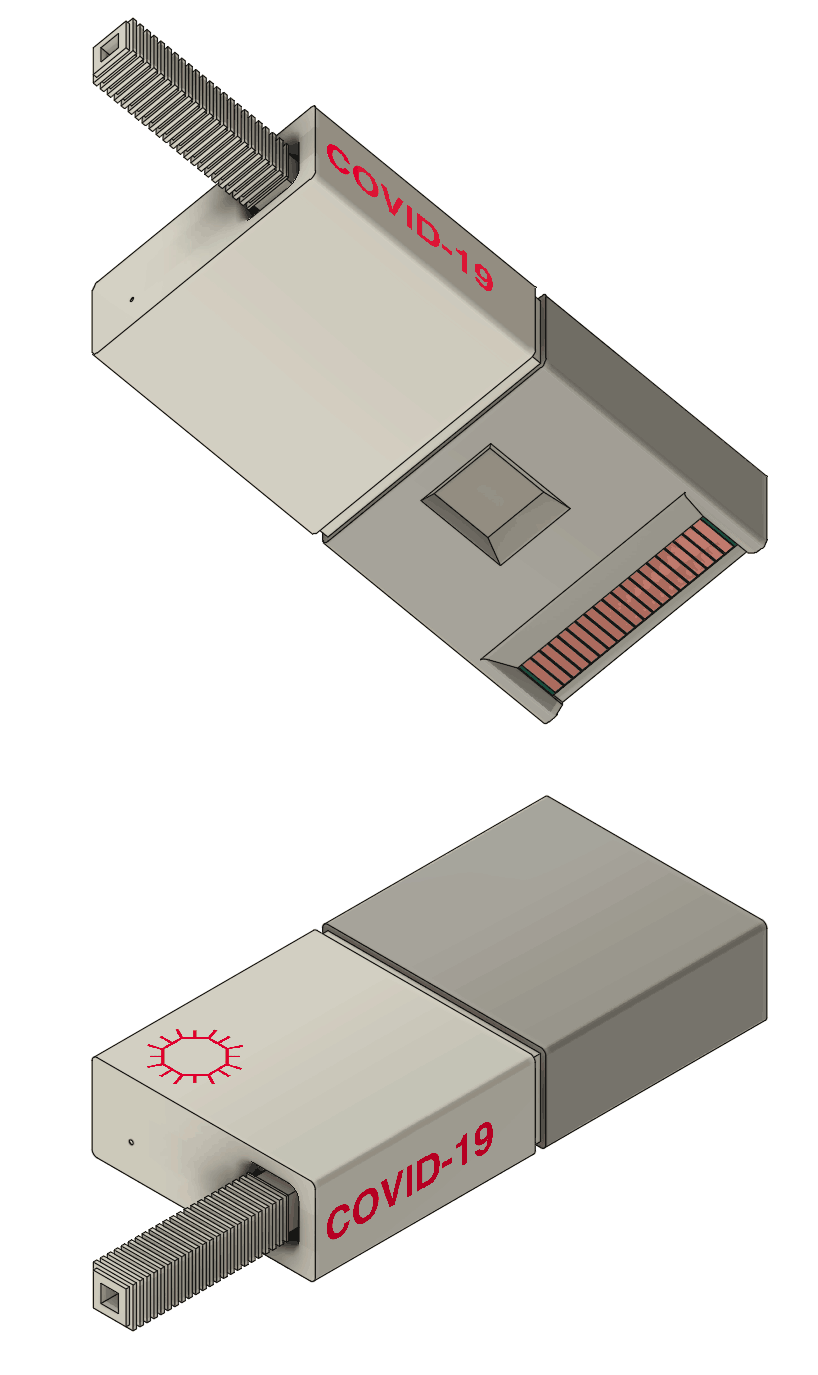
\includegraphics[height=3.3in]{cuetechnicalcolor}  
  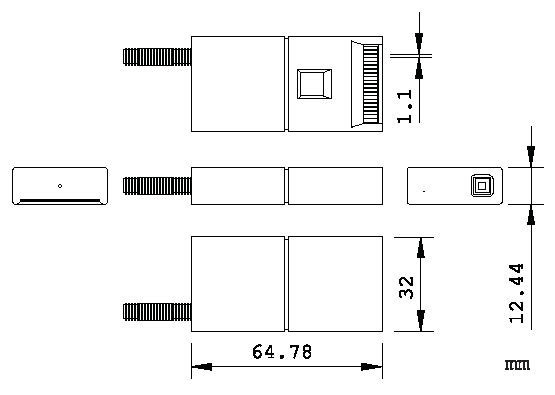
\includegraphics[height=3in]{cuetechnical}
  \caption{ Mechanical drawing of the Cue COVID-19 test cartridge. The
    protruding stick is the nasal swab, which is permanently captured
    during use with zip-tie--like ratcheting. The card edge connector
    is the low tolerance piece here, whose small size (0.05 inch pitch
    with 1.1mm fingers) requires special consideration for mounting
    and soldering. (In its normal usage, this connector mates with
    some spring-loaded pins when the cartridge is inserted in the Cue
    reader.) } \label{fig:cuetechnical}
\end{figure*}

\begin{figure}[ht]
  \centering
  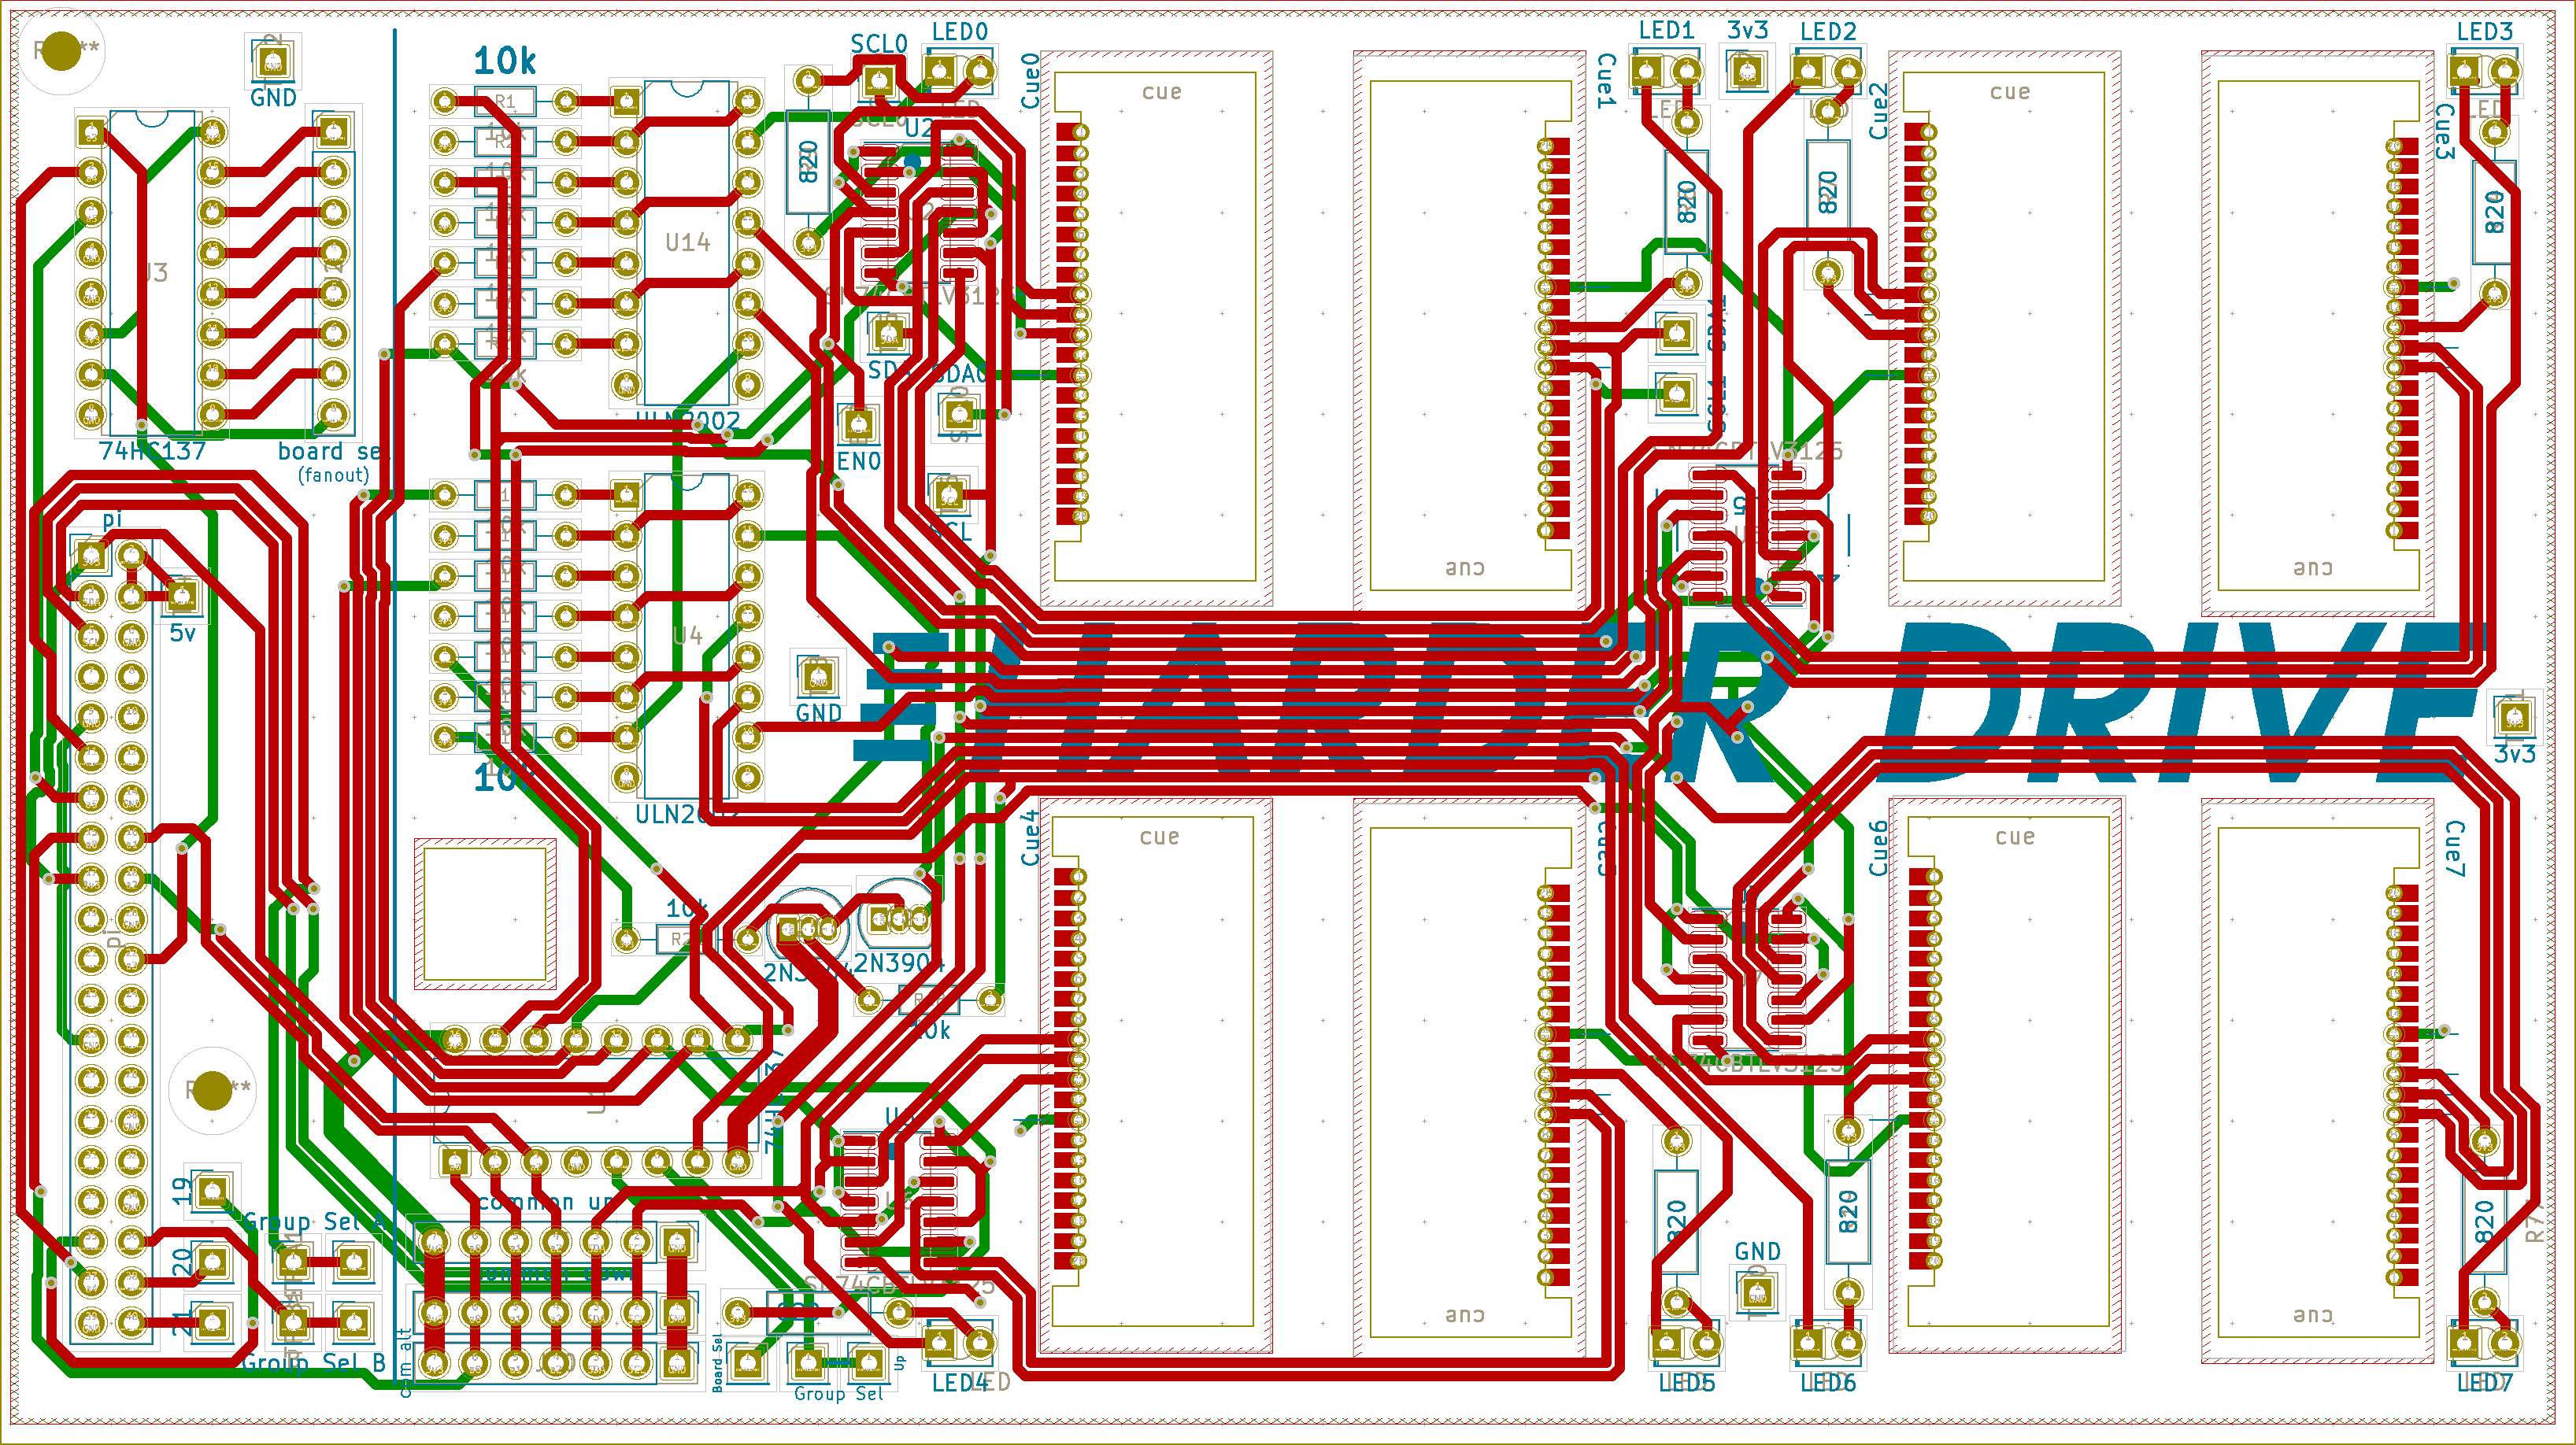
\includegraphics[width=\columnwidth]{pcb}
  \caption{ The two-layer printed circuit board for the Cue drive.
    Because the boards must be ordered in quantity, one board contains
    the layout for both the motherboard (used once) and daughter
    boards (used many times). On the far left is the motherboard, for
    example the header for interfacing with the Raspberry Pi and the
    3:8 demultiplexor for selecting a daughter board. These parts are
    only populated once. The remainder is the daughter board: Eight
    cutouts for cue cartridges mounted at $90^\circ$ with castellated
    edges; an LED and support logic for each; the surface-mount bus
    switch ICs; another 3:8 demultiplexor for selecting the cartridge
    on this board. The design can accommodate 16 daughter boards, each
    with 8 cartridges, for a total of 64 kilobytes. } \label{fig:pcb}
\end{figure}

\newcommand\itwoc{$\textrm{I}^2\textrm{C}$}

The EEPROM is an \itwoc\ device, so I could use pre-existing code to
send commands to it. Reading the EEPROM is normal difficulty. I found
writing to be more like ``hurt me plenty'' difficulty: When you write
a line, the EEPROM drops off the bus temporarily (it may need to do
this because it is internally stepping up voltage for the erase
operation). You then have to either wait ``enough time'' or poll it to
see when it's ready to write the next line. What I did is to
repeatedly try to read back the same line we just wrote (this also
allows us to check that the data were successfully written). However,
sometimes the chip would come online {\em during} the read command,
producing unpredictable results. Basically you have to be tolerant of
errors in some situations, but not {\em too} tolerant, or else you
don't detect real failures. It gives me some sympathy for terrible
dedicated EEPROM programmers I have used~\cite{murphy2018making}.

\subsection{Harder Drive: Cu}

Having committed to the naming scheme where I replace some of the last
letters of the thing with the letter u, it seems the best name for
this drive is {\tt Cu}. For one thing, this is the chemical symbol for
copper, and the drive uses copper to function.

With the ability to read and write a single Cue cartridge, the
remainder is just a matter of straightforward engineering and tedious
manual labor. Of course, you want to do all of this on a manufactured
printed circuit board (Figure~\ref{fig:pcb}). The job here is to make
it possible to individually address a single EEPROM to read and write
its data. Though \itwoc\ does support multiple devices on the same
bus, these chips all have the same \itwoc\ address and so they would
all try to reply to the same commands. The ST 24C04WP EEPROM does have
``chip enable'' pins that would allow it to share a bus with others,
by selectively enabling only the chip of interest. Unfortunately,
these pins are not connected to any of the exposed connectors on the
cartridge. Instead, I use a bus switch (which is basically this same
``chip enable'' circuitry) to connect each EEPROM to the \itwoc\ bus.
Each SN74CBTLV3125 is a quad bus switch, so I can switch the two
\itwoc\ lines (SDA, SCL) for two Cue cartridges with each chip. Then,
we can select one of 8 cartridges (a single daughter board) with a
demultiplexor, which takes 3 address bits and sets exactly one of its
8 output lines to {\tt 0}. For decorative purposes, I associate a
colored LED with each cartridge; this LED foolishly ends up accounting
for most of the components on the board and most of the assembly time,
since I also have to build logical NOT gates (demultiplexor outputs
logical {\tt 0}). Finally, the cartridges themselves are very tricky
to incorporate. They have very small plated connectors that normally
mate with spring-loaded pins in the reader, but that component is not
readily available (and would probably be expensive). Instead, I mount
it at $90^\circ$ through a hole in the PCB, where the PCB has its own
matching edge connector made with castellated holes. I also 3D printed
a plastic jig that could hold the cartridge at the right angle during
soldering. With generous acid flux and a steady hand, soldering these
worked quite well. Only 4 pins need to be connected (3v3, GND, SDA,
SCL) but I also soldered some distal pins, since these joints are the
only mechanical connections for the cartridges.

The motherboard has its own demultiplexor to select the daughter
board, as well as an ad hoc pair of ``group selector'' pins wired
directly to GPIO. Together it supports 7-bit addresses, for up
to 128 cartridges, which is 64~kilobytes. I did not collect enough
used tests to fill the address space, but I did connect 72 of them,
which is enough to do something interesting at least! Except \ldots

\subsection{Failure!} \label{sec:failure}
\noindent

\includegraphics[width=\columnwidth]{failure}

I blew it! Literally! On the evening of the SIGBOVIK deadline, in an
attempt to be simultaneously {\em expedient} and {\em careful}, I
soldered the Cu motherboard while it was plugged in, and fully toasted
it and the connected Raspberry Pi. My best guess is that the soldering
iron had a very different idea of ``ground'' than the device under
test. It made an upsetting pop noise, an upsetting burn smell, an
upsetting spark and smoke sight, an upsettingly warm touch,\footnote{
  I did not attempt to taste it; the board is not RoHS-compliant due
  to the copious lead used. Despite the panoply of upsetting
  sensations, the obviousness of the failure was a blessing that saved
  me time trying to debug! Even if I plug the Pi in on its own, it
  makes a pathetic, obviously unhealthy whine. It is so dead.} and it
made it impractical to fix before the paper is due. You can at least
see what the tabletop device looks like in Figure~\ref{fig:cu}. It
should be possible to replace the Pi and motherboard, so perhaps the
by the accompanying video or talk I will be able to finish the task
and get some benchmark numbers.

\begin{figure}
  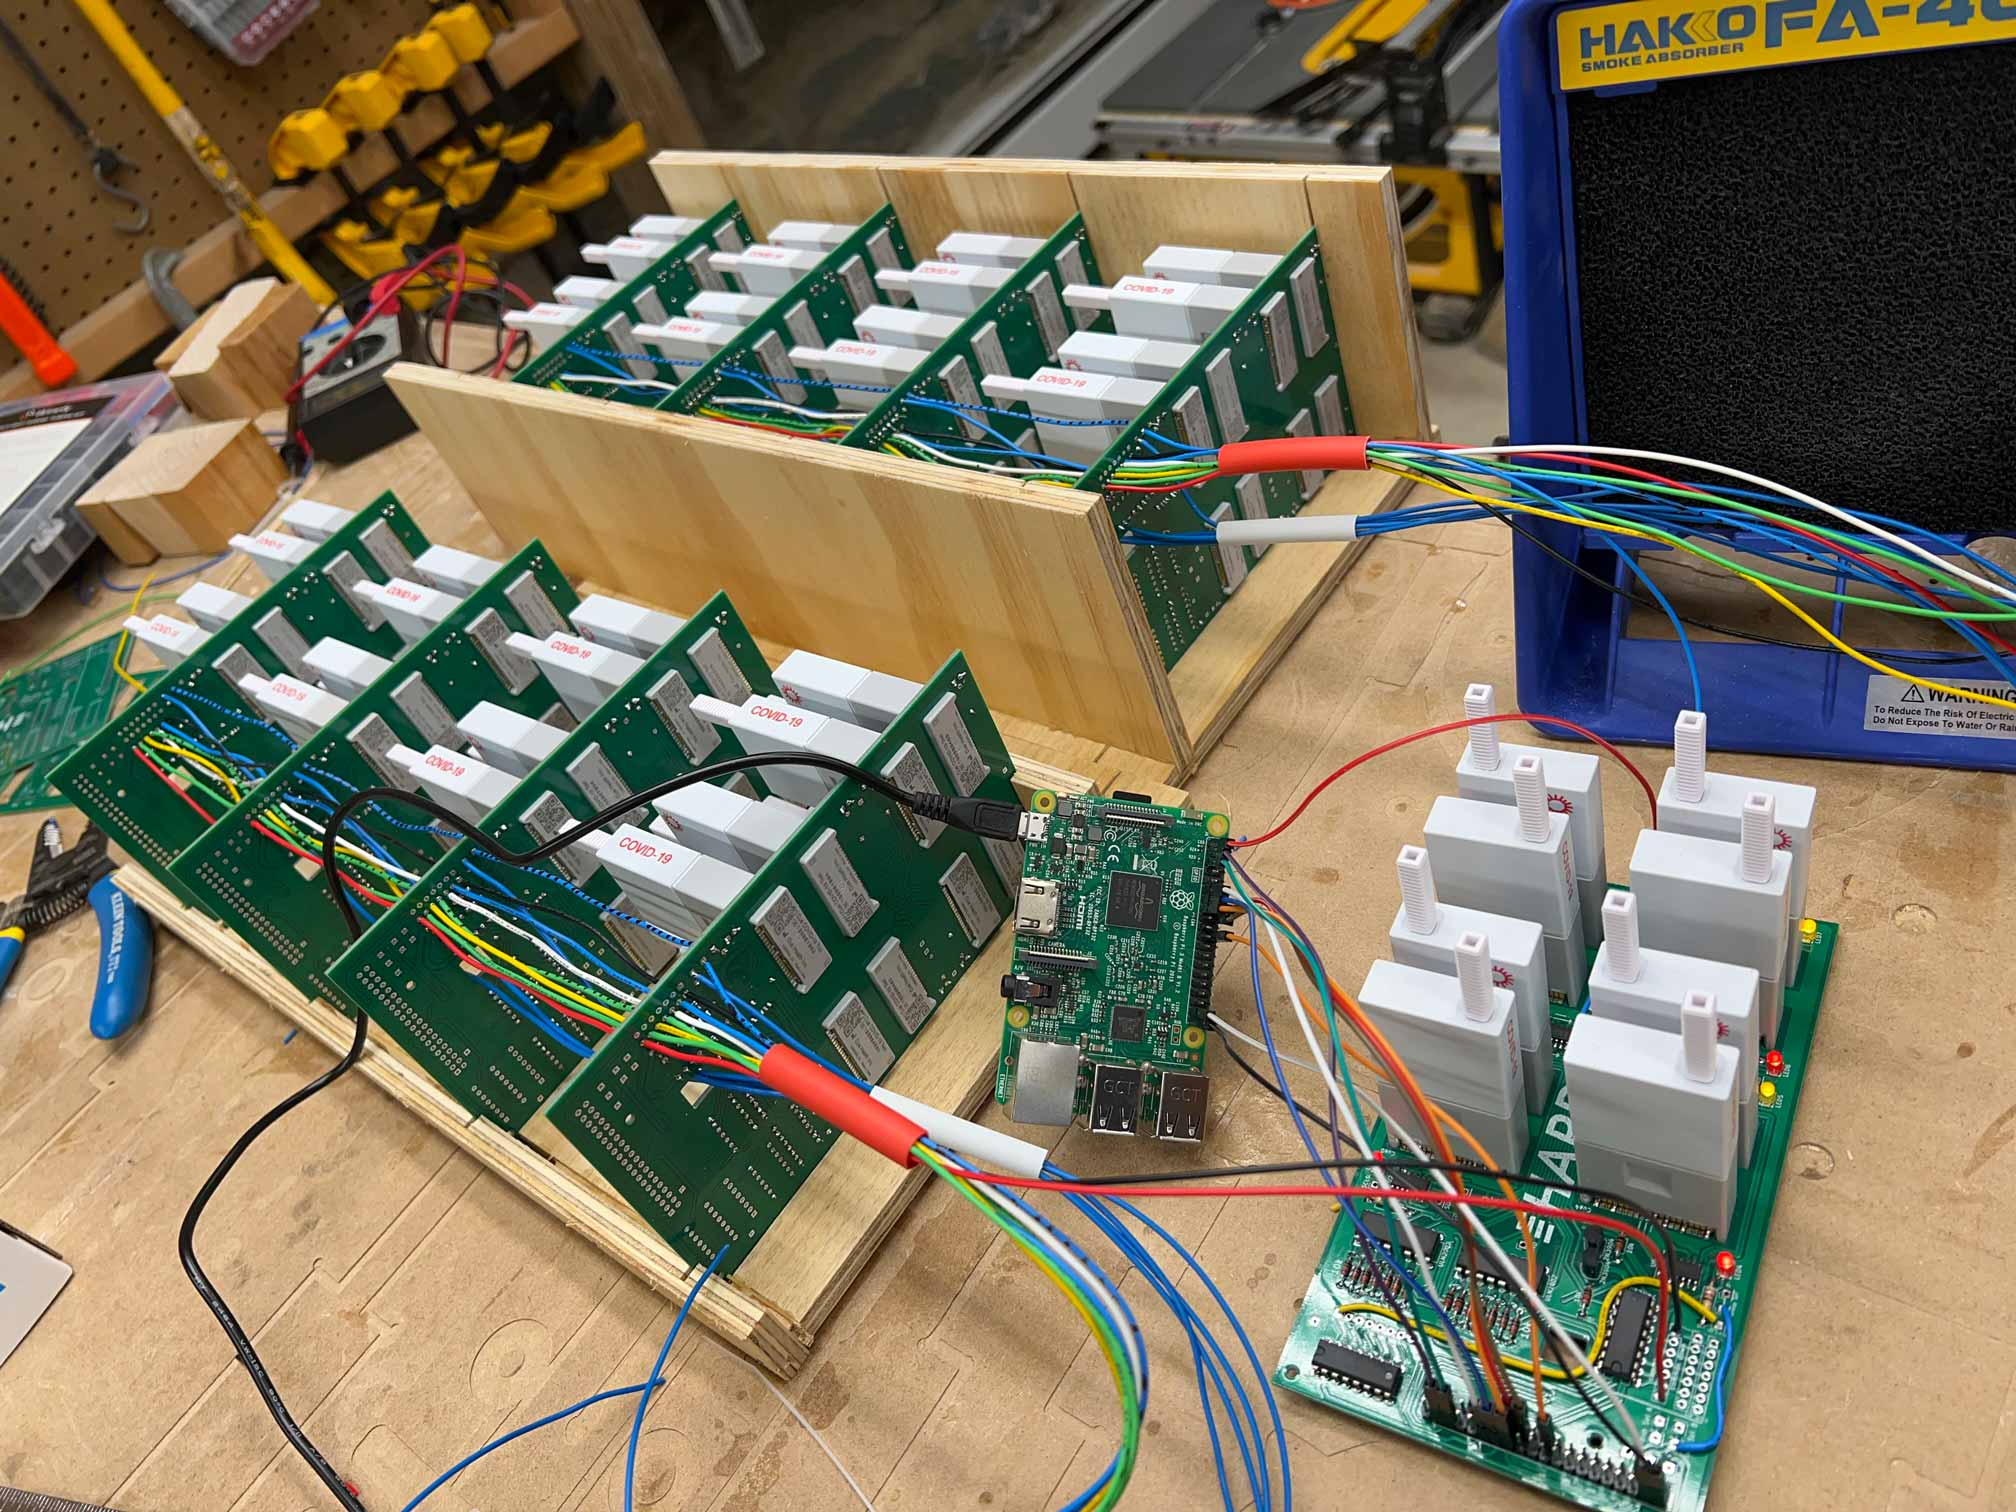
\includegraphics[width=\columnwidth]{cu}
  \caption{
    Assembled {\tt Cu} drive with 72 Cue cartridges. Imagine
    trying to explain to someone that this homemade thing
    that has ``COVID-19'' written on it 72 times, and
    has got all sorts of colored wires everywhere, is not
    some instrument of bioterror. In fact it does not even
    drive hard: In my rush to meet the preposterously strict
    SIGBOVIK deadline, I fried the Raspberry Pi {\em and}
    motherboard (perhaps you can see that multiple LEDs are
    lit on the motherboard, which clearly violates invariants).
    Fortunately due to its modular design, it can likely be fixed
    with a few more hours of manual labor.
  } \label{fig:cu}
\end{figure}

\subsubsection{Results}

We need a file to store on the drive to tie the knot and to run the
benchmark. A beautiful choice here is the genetic sequence of
SARS-CoV-2 (ancestral)~\cite{sarsncov2sequence} from
GenBank~\cite{clark2016genbank}. This is a 77343 base-pair sequence;
it would be too large to store in ASCII.\footnote{Plus, I'm a biology noob
  and I may just be missing something, but GenBank uses ``T'' in
  this sequence even though it should be U (uracil) in RNA, which seems
  very non-canonical?} Each nucleotide is only two bits of information,
though, so we pack four of these into each byte for only 19336 bytes.

\paragraph{Qualitative.} This is a decent Harder Drive. It solves a problem
we don't have, which is what to do with all those COVID-19 tests that
we'd otherwise just throw away? It took significant effort to create,
although most of the difficulty was from problems (e.g.~how to solder
these tiny pins) that are not interesting from a computer science
perspective. EEPROMs are fundamentally data-storage devices, so this
usage of them cannot be considered clever, but arraying dozens of
them to create a modest-sized non-volatile memory that could be easily
replaced with a single 30-cent NAND Flash IC is at least ``very silly.''
Mucho demerits because I broke it during the final assembly.

\paragraph{Cost.} The cost is significant. The up-front cost is
a Raspberry Pi 3 (nominally \$35), accessories, and a demultiplexor IC
(\$0.60), plus scrap plywood for mounting. Then, per board, we have
the following bill of materials:

\smallskip
{
  \renewcommand{\tabcolsep}{2pt}  
  \scriptsize
  \noindent
  \centering
\begin{tabular}{@{}rllll@{}}
{\bf Qty.} & {\bf Part no.}  & {\bf Description}  & {\bf Price ea.} & {\bf Total}   \\
\hline
& & & & \\[-0.5em]
8    & Cue L2900006  & Used COVID-19 Test     & \$65.00     & \$520.00 \\
1    & custom        & 2-layer PCB 162x92mm   & \$5.766     & \$5.766 \\
2    & 497-2340-5-ND & Transistor array IC    & \$0.5768    & \$1.154 \\
4    & SN74CBTLV3125 & Bus switch IC          & \$0.6636    & \$2.654 \\
2    & 2N3904        & NPN BJT transistor     & \$0.09      & \$0.18 \\
20   & jellybean     & 10k$\Omega$ resistor   & \$0.0155    & \$0.31  \\
8    & jellybean     & 845$\Omega$ resistor   & \$0.02428   & \$0.194 \\
8    & jellybean     & 3mm LED 2v 20mA        & \$0.01499   & \$0.12  \\
1    & CD74HC137E    & 3:8 demultiplexor IC   & \$0.6048    & \$0.605 \\
\hline
& & & & \\[-0.5em]
&               &                      &    & {\normalsize \$530.98} \\
\end{tabular}
  % perhaps should have "saved" the old value?
  \renewcommand{\tabcolsep}{6pt}  
}
\smallskip

This does not include consumables like solder and hook-up wire, nor the
considerable time to assemble each board (about 1 hour with practice).

We need 13 boards to store a full FAT12 filesystem, for a total cost
of \$6,936.04. The marginal price per byte is 12.96 cents.

\paragraph{Longevity.} This is the only drive considered where data
are retained when powered down. The M24C04-W EEPROM is rated for 200
years of data retention, and 4 million write cycles~\cite{stm24c0w}.
At the current pace, this is likely to outlast the human race.

\paragraph{Speed.} Unknown as of publication! As described in
Section~\ref{sec:failure}, the motherboard was damaged on the eve of
the deadline and no benchmark was conducted. Reading the EEPROM is
fast, but writing a block takes a few hundred milliseconds. The speed
is expected to be high (for the drives considered here).

\paragraph{Power.} The up-front power cost is low; we need to power
the Raspberry Pi and various chips on the boards. Only one of the
decorative LEDs is lit at a time, using about 1~mW. The total is about
3~Watts. % XXX actually measure it, though.
The marginal power cost is excellent: On the Cue cartridge,
only the EEPROM is powered. During standby it uses no more than
3~$\mu$A at 3.3~V, which is 9.9~$\mu$W for 512 bytes, or 19.3~nW per
byte.

\paragraph{Is rotational?} This drive is not rotational; it provides
us SSD-like random access to the Cue cartridges, and the EEPROMs on
board allow random access to each line of data.

\paragraph{Harm to society.} Arguably, the drive is beneficial to
society. First, it is built mostly from trash. Second, coronavirus
testing prevents death or other hardship by informing infected people
that they may be contagious; at a minimum it is good for the spirit by
facilitating lower-anxiety gatherings. Finally, since the tests
contain captured body fluids, this adds an all-too-rare ``human
element'' to computing.


\section{Other hard drives we really didn't need}

Here are some things I hate: (1) The name of TDAmeritrade's stock
trading app, which is ``thinkorswim.'' This is of course a play on the
idiom to ``sink or swim,'' meaning metaphorically to toss someone into
deep water to survive by their own efforts, or else drown. The analogy
is certainly apt for an app that lets consumers trade derivatives, but
the obvious problem here is that if it is ``think or swim,'' then we
are now asking the subject to survive by their own efforts (swim) or
else ``think''? Huh? Or is it that they must think carefully about
their trades, or else they will survive? Wha? \quad (2) Poison ivy.
This plant has no purpose other than to make you itch. It doesn't even
get anything out of that trick, since I wasn't going to eat it anyway.
Nevertheless it spreads. \quad (3) Cryptocurrency. I have no objection
to the use of cryptography in finance, but there aren't enough
vomiting emojis in Unicode to appropriately react to the current hype.
Cryptocurrency significantly harms the planet while taking advantage
of many people's technical and financial illiteracy.\!\footnote{ Note
  to cryptocurrency apologists: This short section does not have room
  for a full criticism, nor would such a thing be ``fun'' enough for
  SIGBOVIK. Briefly, there are five principal problems. (1) Proof of
  Work is incredibly wasteful (see the stats below; this is just {\em
    one} of the cryptocurrencies). Of course I am aware of ``Proof of
  Stake.'' I remain very skeptical that miners with large capital
  investments in (otherwise useless) ASICs will be willing to salvage
  them, but I would gladly celebrate this and by all means, please do
  make this happen. (2) I believe that regulation of finance is {\em
    good}, both formal regulation with law and self-regulatory
  organizations like FINRA, as well as informal practices like rolling
  back erroneous transactions or returning stolen funds, which are
  regulated indirectly by the desire to maintain valuable public
  reputations. Unregulated markets have many problems (insider
  trading, etc.) and avoiding regulation mostly seems to be useful for
  tax evasion and other crimes. (3) In attempt to avoid
  ``decentralization'', control is nonetheless effectively centralized
  in the hands of a small number of actors anyway (large-capacity
  miners and exchanges). However, these actors are set up as
  adversarial, or at best as some kind of wild-West ``disruptors.''
  I'd trust these skeezy guys way less than I trust banks, and rightly
  so: They routinely front-run transactions, just as one example. (4)
  The space is riddled with Ponzi schemes and scams, as exemplified
  (but certainly not limited to) NFTs. This is plainly immoral. (5)
  Cryptocurrency aficionados are insufferable, presumably because they
  feel like they need to convince you to get in on their tokens so
  that they grow in value (which presumably they hope to then sell to
  get real money). I get an enormous amount of cryptocurrency spam.
  The only words I've muted on Twitter other than five green Unicode
  squares are cryptocurrency terms, and this has improved the
  experience greatly. If you are a cryptocurrency aficionado reading
  this that feels like you need to ``educate'' me about how I am
  misinformed (despite what I can clearly see in front of me!), case
  in point. That said, I will happily discuss interesting ideas with
  informed computer scientists over beer. }

Nonetheless, the common prefix between ``block device'' and
``blockchain'' is hard to avoid noticing, and a head-to-head
comparison may be instructive. So I put on incognito mode, a VPN, an
N-95 mask and six condoms in order to research some numbers for this
section.

Bitcoin is ``append-only'' by design, so it does not have the same
abstraction as other Harder Drives. For comparison sake, we consider a
usage where the head of the blockchain contains the full data; a write
is accomplished by mining a new block and a read is accomplished by
reading from the current head. For Bitcoin, the block size is 1~Mb,
and the network automatically adjusts to mine a single block every ten
minutes. I did {\em not} actually implement this drive, both because
of the gag reflex and because I do not have that kind of money!

\paragraph{Qualitative.} Despite hating it, I must admit that Bitcoin
meets the criteria for a Harder Drive pretty well. It solves a problem
that we don't have, by imagining a world where we cannot agree on a
small set of trustworthy parties, a majority of which must be acting
in good faith. Its approach is elegant in the small but for its
obvious fatal flaws, and comically absurd if taken to its logical
extreme. It is impressively inefficient, and grows less efficient over
time. In short, it would make a solid SIGBOVIK paper. The only problem
is that people are actually using it in seriousness, and the social
problems that result from the value it has attained.

\paragraph{Cost.} The cost is extremely high. The reward for mining
one Bitcoin is currently 6.25~BTC, plus an average of about 0.97~BTC
% 47577 on 28 Mar 2022
in transaction fees, which totals \$342,000 in March 2022. This gives
us an approximate upper bound on the cost to mine (by assuming the
marginal cost is profitable) a block, which is 34.2 cents per byte.
This does not include the up-front cost of hardware and facilities,
which is of course monumental.\!\footnote{Nor the surrounding
  apparatus like ``bitcoin ATMs'' and ``crypto exchanges'' (the kind
  of stuff that apologists are talking about when they tell you that
  ``regular money uses a lot of electricity too!''), although it is
  probably not fair to count these as part of the cost when used as a
  pure data storage mechanism.}

\paragraph{Longevity.} The data has excellent longevity, in fact, it
is impossible to erase previous data once written. Of course,
``forks'' of the chain can make it unclear what version of the data is
correct, or if $>50\%$ of the untrusted miners disagree, they can
change the data at will.

\paragraph{Speed.} The network is slow, although not the slowest considered
here. It takes an expected ten minutes to write 1~Mb of data. This is
a data rate of 1,747~bytes/sec, approximately the speed of a
14.4~kbaud modem.

\paragraph{Power.} The power usage is incredibly high. Mining Bitcoins
uses about 0.31\% of the entire world's energy production,
15.74~GW~\cite{cbeci}. Remember that this does not solve any
interesting computational problems or accomplish anything useful; the
only purpose is to create an expensive waste of power in order to
avoid trusting a bank or set of banks. To store one megabyte on an
ongoing basis, this is 15.74~kW per byte.

\paragraph{Is rotational?} It's not even rotational!

\paragraph{Harm to society.} The harm to society is significant. Aside
from the catastrophic waste of resources, the primary use case is
speculation (at best morally neutral, but probably tends to harm small
investors). As a slow, expensive, non-atomic yet irrevocable payment
mechanism, they are best suited for extortive transactions like
Ransomware.

\section{Conclusion}

In this paper, we decided that sometimes it's more fun to do things
the hard way, and then did so. Using several different techniques and
some needless digressions, we created block devices that could support
small filesystems, which then could host a fitting file. Each
filesystem was bad when considered as a regular hard drive, but good
when considered as a Harder Drive. We also compared these drives to
the most popular cryptocurrency. The idea was to make the point that
cryptocurrency is so egregiously bad that it resembles a ``SIGBOVIK
joke gone wrong'' more than something one would make on purpose. This
part may not have been as fun.

\paragraph{Acknowledgements.}

I used {\tt nbdkit}~\cite{nbdkit} to create block devices, which was a
much sounder idea than writing my own kernel drivers. I still found it
very easy to render Linux unusable. The code for sending and receiving
pings was adapted from {\tt liboping}~\cite{liboping}.

Thanks to Rose, William, Sophia, Reed, Jessica, Max, and Finn for
donating their nasal swabs to the project. I especially appreciate
that they gave me these samples without any information about what I
was even doing with them. That's true friendship. By the way, human
cloning is possible now. Just sayin'.

If you have a computer connected to the internet, then I attempted
to send it a message during the course of this project. If your
computer responded, then thank you for configuring it that way.
Similarly, this paper would like to acknowledge any TCP SYN packets
that are sent to it (but it cannot, for it is simply a paper).

Finally I would like to thank the SIGBOVIK program committee for letting
me store this file in the proceedings:

% tar  -c -M  --record-size=2560 --tape-length=2953c --new-volume-script='echo out${TAR_VOLUME}.tar >& ${TAR_FD}' --file=out1.tar QR_code.bz2
% (I think I actually ended up using the 'split' command, though?)

\startsquarepar
\noindent

\includegraphics[height=1.7in]{q01}

\includegraphics[height=1.7in]{q02}

\includegraphics[height=1.7in]{q03}

\includegraphics[height=1.7in]{q04}

\includegraphics[height=1.7in]{q05}

\includegraphics[height=1.7in]{q06}

\includegraphics[height=1.7in]{q07}

\includegraphics[height=1.7in]{q08}

\includegraphics[height=1.7in]{q09}

\includegraphics[height=1.7in]{q10}

\includegraphics[height=1.7in]{q11}

\includegraphics[height=1.7in]{q12}

\includegraphics[height=1.7in]{q13}

\includegraphics[height=1.7in]{q14}
\stopsquarepar

\bibliography{pingu}{}
\bibliographystyle{plain}

\end{document}

